%\newpage
\subsection{Подготовка производства}
\label{bp:Prepare}
%

Клиент присылает требования на изготовления продукции в любом виде. Некоторые клиенты высылают готовую спецификацию (рис. \ref{pic:1.1 спецификация от контрагента_0001}). Опросного листа не выявлено.
Заказчики могут предоставить образец продукции, по которому менеджер производит замеры  или может выполнить расчет размеров короба по готовой продукции. В случае, если менеджер не может точно ответить на запросы клиента, то он обращается к главному технологу по электронной почте (рис. \ref{pic:1.11 запрос от менеджеров к технологу_0001}) или по телефону. 

Менеджер рисует в системе 1С:УПП макет (форма \ref{pic:d8}).
 Менеджер рисует в редакторе Paint вручную размеры, технологические отверстия, мануальные знаки. Также менеджеры рисуют макет на сложную высечку.   Технологи макеты не создают.
 Менеджер в редакторе Paint рисует макет и отправляет клиенту на согласование (форма \ref{pic:d9}).  Технологический отдел в этом процессе не участвует.

% По запросу от менеждера технолог рассчитывает площадь печати и площадь изделия. Расчеты производятся в MS Excel. Главный технолог рассчитывает стоимость печати и сообщает менеджеру. По данным от главного технолога менеджер рассчитывает окончательную цену продукции и сообщает ее клиенту.
% % (рис. \ref{pic:a8}, \ref{pic:a9}). 

Технологические карты создаются в 1С:УПП. Созданию ТК предшествует создание макета. Если изделие без печати, то макет создает сам менеджер (рис. \ref{pic:1.7.2 Макет от менеджера_0001}). При наличии печати макет по запросу от предприятия создает ООО "Аверс" (рис. \ref{pic:1.7.1 дизайн от Аверс_0001}). Все макеты проверяет главный технолог. Если есть замечания, то главный технолог возвращает макет на доработку (рис. \ref{pic:1 Замечания технолога в ТК}). После исправления всех замечаний главного технолога, менеджер отправляет макет на согласование и подпись клиенту (рис. \ref{pic:1.7.3 подписанный макет_0001}). Отдельно готовая технологическая карта с клиентом не согласовывается.

Менеджер создает технологическую карту (рис. \ref{pic:0 ТК в УПП_0001}). Менеджер определяет маршрут для производства продукции используя специальную форму в системе 1С:УПП (рис. \ref{pic:0 определение маршрута_0001}). В системе 1С:УПП для менеджеров созданы справочники, по рилевкам, упаковке (рис. \ref{pic:1.7.5 схемы упаковки_0001}), схемам укладки, размерам ящиков (рис. \ref{pic:1.7.4 справочник для маршрутов_0001}) и т.д.  Главный технолог проверяет технологические карты на наличие ошибок. В системе 1С:УПП технолог утверждает технологическую карту и только после этого технологическая карта может быть использована при выработке заказов. Главный технолог фиксирует факт проверки ТК у себя только в бумажном виде (рис. \ref{pic:1.7.4 список проверенных ТК_0001}).
Удаление технологических карт производится менеджерами. Главный технолог доступа к журналу (списку) технологических карт не имеет. 

В системе 1С:УПП менеджер передаёт статус передать технологу, вернуть менеджеру, утвердить.
Менеджер согласовывает бизнес-карту в системе 1С:УПП, где рассчитывается нормативная себестоимость изделия, согласовывает либо с начальником отдела продаж, либо с генеральным директором.


Общее количество технологических карт на предприятии не установлено. 


%В производстве и в отделе подготовки производства технологические карты пользователи ищут по размерам изделия и по наименованию контрагента, что может привести к ошибке. 

% Новых изделий ОПП заводят от 2 до 40 шт в день. 
% Пример полного комплекта технологической карты приведен на форме \ref{pic:a5}.
%Требования по новому изделию хранятся локально у МАП на компьютере или в почте. 

%%
%После согласования цены на основании калькуляции (рис. \ref{pic:d1}) МСЗ создает в таблице MS Excel техническое задание для дизайнера по шаблону. 
%МСЗ в сети создает папку с новым номером изделия из 4 цифр. МСЗ создает новое техническое задание на разработку нового изделия, присваивает новый номер. 
%Номер технологической карты --- это номер карты раскроя (рис. \ref{pic:d7}).
%Номер ТК МСЗ переносит в калькуляцию вручную. Номер МСЗ указывает в форме спецификации (рис. \ref{pic:d6}). 
%По наличию номера в печатной форме технологической карты МСЗ проверяет ее наличие.
%МСЗ отправляет клиенту проект договора, спецификацию к договору и список технологических карт.
%МЗС сохраняет предоставленные клиентом файлы в папку с технологическими картами. 

%После согласования цены на основании калькуляции (рис. \ref{pic:d1}) МСЗ создает в таблице MS Excel техническое задание (рис. \ref{pic:d7}) на разработку технологической карты дизайнеру и сохраняет в папке с номером ТК. Номер присваивает МСЗ и создает папку с новым номером изделия из 4 цифр.
%Номер технологической карты --- это номер карты раскроя (рис. \ref{pic:d7}).
%Номер ТК МСЗ переносит в калькуляцию вручную. Номер МСЗ указывает в форме спецификации (рис. \ref{pic:d6}). 

%Менеджер при приемке нового изделия согласовывает возможность изготовления продукции по таблице (рис. \ref{pic:d28}). 
%Если есть вопросы по изготовлению, то  менеджер создает вопрос в техотдел. 
% (рис. \ref{pic:d28}).

%При поступлении заявка на производство от отдела продаж %(рис. \ref{pic:d2}) с пометкой «новая» в технологическом отделе сотрудники начинают разработку новой технологической карты (ТК).

%Разработкой ТК на четырехклапанный короб занимается инженер-конструктор технологического отдела. В шаблон ТК таблицы MS Excel инженер указывает  размеры четырехклапанного короба %(рис. \ref{pic:a2}) и через формулы просчитывает необходимые параметры. Инженер создает ТК на четырехклапанный короб. Папка с созданными ТК на четырехклапанные короба хранится на сервере.
% (рис. \ref{pic:a1}). 
%Папки разделены по клиентам. При отсутствии папки по клиенту менеджеры создают нового клиента и новую ТК. 

%Отдельно от ТК инженер ОПП разрабатывает схему упаковки и расчет укладки на поддон  в формате MS Excel (рис. \ref{pic:f3}). Схемы укладки хранятся отдельно в папке на сервере (рис. \ref{pic:d26_1}). 

%Также в технологическом отделе разрабатывают бирку на ГП и их хранят тоже отдельно в папке на сервере (рис. \ref{pic:a4}).

%При разработке нового дизайна менеджер присылает письмо на электронную почту художнику-конструктору с требованием о разработке дизайна нового изделия. 
%Художник-конструктор разрабатывает макет на основании данных присланных в письме, готовый макет высылает менеджерам для согласования с клиентом. 
%После согласования макета с клиентом художник-конструктор делает заказ клише в «Колор Стандарт Сервис» (см. процесс ''Учет %технологической оснастки и краски'' \ref{bp:rigging}). Сканы подписанных клиентом макетов с дизайном хранятся на сервере в папках в сетевом доступе. % ф 3,4. 
%Художник-конструктор разрабатываем макеты в пакете CОRЕL DRAW. 

%Разработку конструкции сложной высечки выполняет инженер-конструктор. 
%Инженер-конструктор разрабатывает макет высечки в пакете AutoCAD (рис. \ref{pic:f10}). На предпритии в ходе обследования выявлена база наработок, чертежей, которые хранятся в сети. % ПК ф.12. 
%Макет конструкции инженер-конструктор согласовывает с клиентом через менеджера. 
%Согласованный чертеж инженер-конструктор отсылает в «РастрТехнологии» (см. процесс ''Учет технологической оснастки и краски'' \ref{bp:rigging}), где чертеж проверяют и наносят «шапку» % ф. 11, 
%и с присвоенными данными по чертежу высылают макет назад. Изготовитель штампа также высылает счет. %, после чего заказывается штамп. 
%Готовые чертежи хранят на сервере. 
%На сложную высечку ТК  хранятся отдельно.

%При изменении в ТК старая форма изымается из производства. 
%Технологичекие карты в печатном виде хранятся на участоке вырубных форм (рис. \ref{pic:f5}). % Ф. 6,7 ТК редко используемые хранятся отдельно. 



\clearpage

%МСЗ сообщает дизайнеру о появлении технического задания.
%В техническом задании МСЗ  указывает тип изделия и внутренние размеры. Заказчик может предоставить уже готовый чертеж, тогда МЗС  прикладывает дизайн от клиента. 
%Созданное техническое задание на разработку изделия МСЗ  высылает дизайнеру на почту. 
%Дизайнер разрабатывает ТК для основных изделий: гофроящик, лоток, решетка, гофролист.
%Дизайнер разрабатывает ТК по запросу (рис. \ref{pic:d8}) в системе Corel Draw. Размеры изделия дизайнер указывает в программе Corel Draw по факту в миллиметрах. Дизайнер разрабатывает только простые изделия и макет печатной формы, выполняет расчет размеров заготовки вручную, в следствие чего существует большая вероятность появления ошибки. Дизайнер вручную рассчитывает размер поддона, рисует схему погрузки продукции в транспорт.

%Дизайнер при необходимости разрабатывает дизайн печати на изделии. 
%Дизайнер в программе Corel Draw рисует коробки, решетки для изготовления штанц-формы. Разработка конструкции сложной высечки не выполняется.
%После разработки макета технологической карты дизайнер сообщает МСЗ о ее готовности по телефону или мессенджеру.

\begin{figure}
\begin{center}
  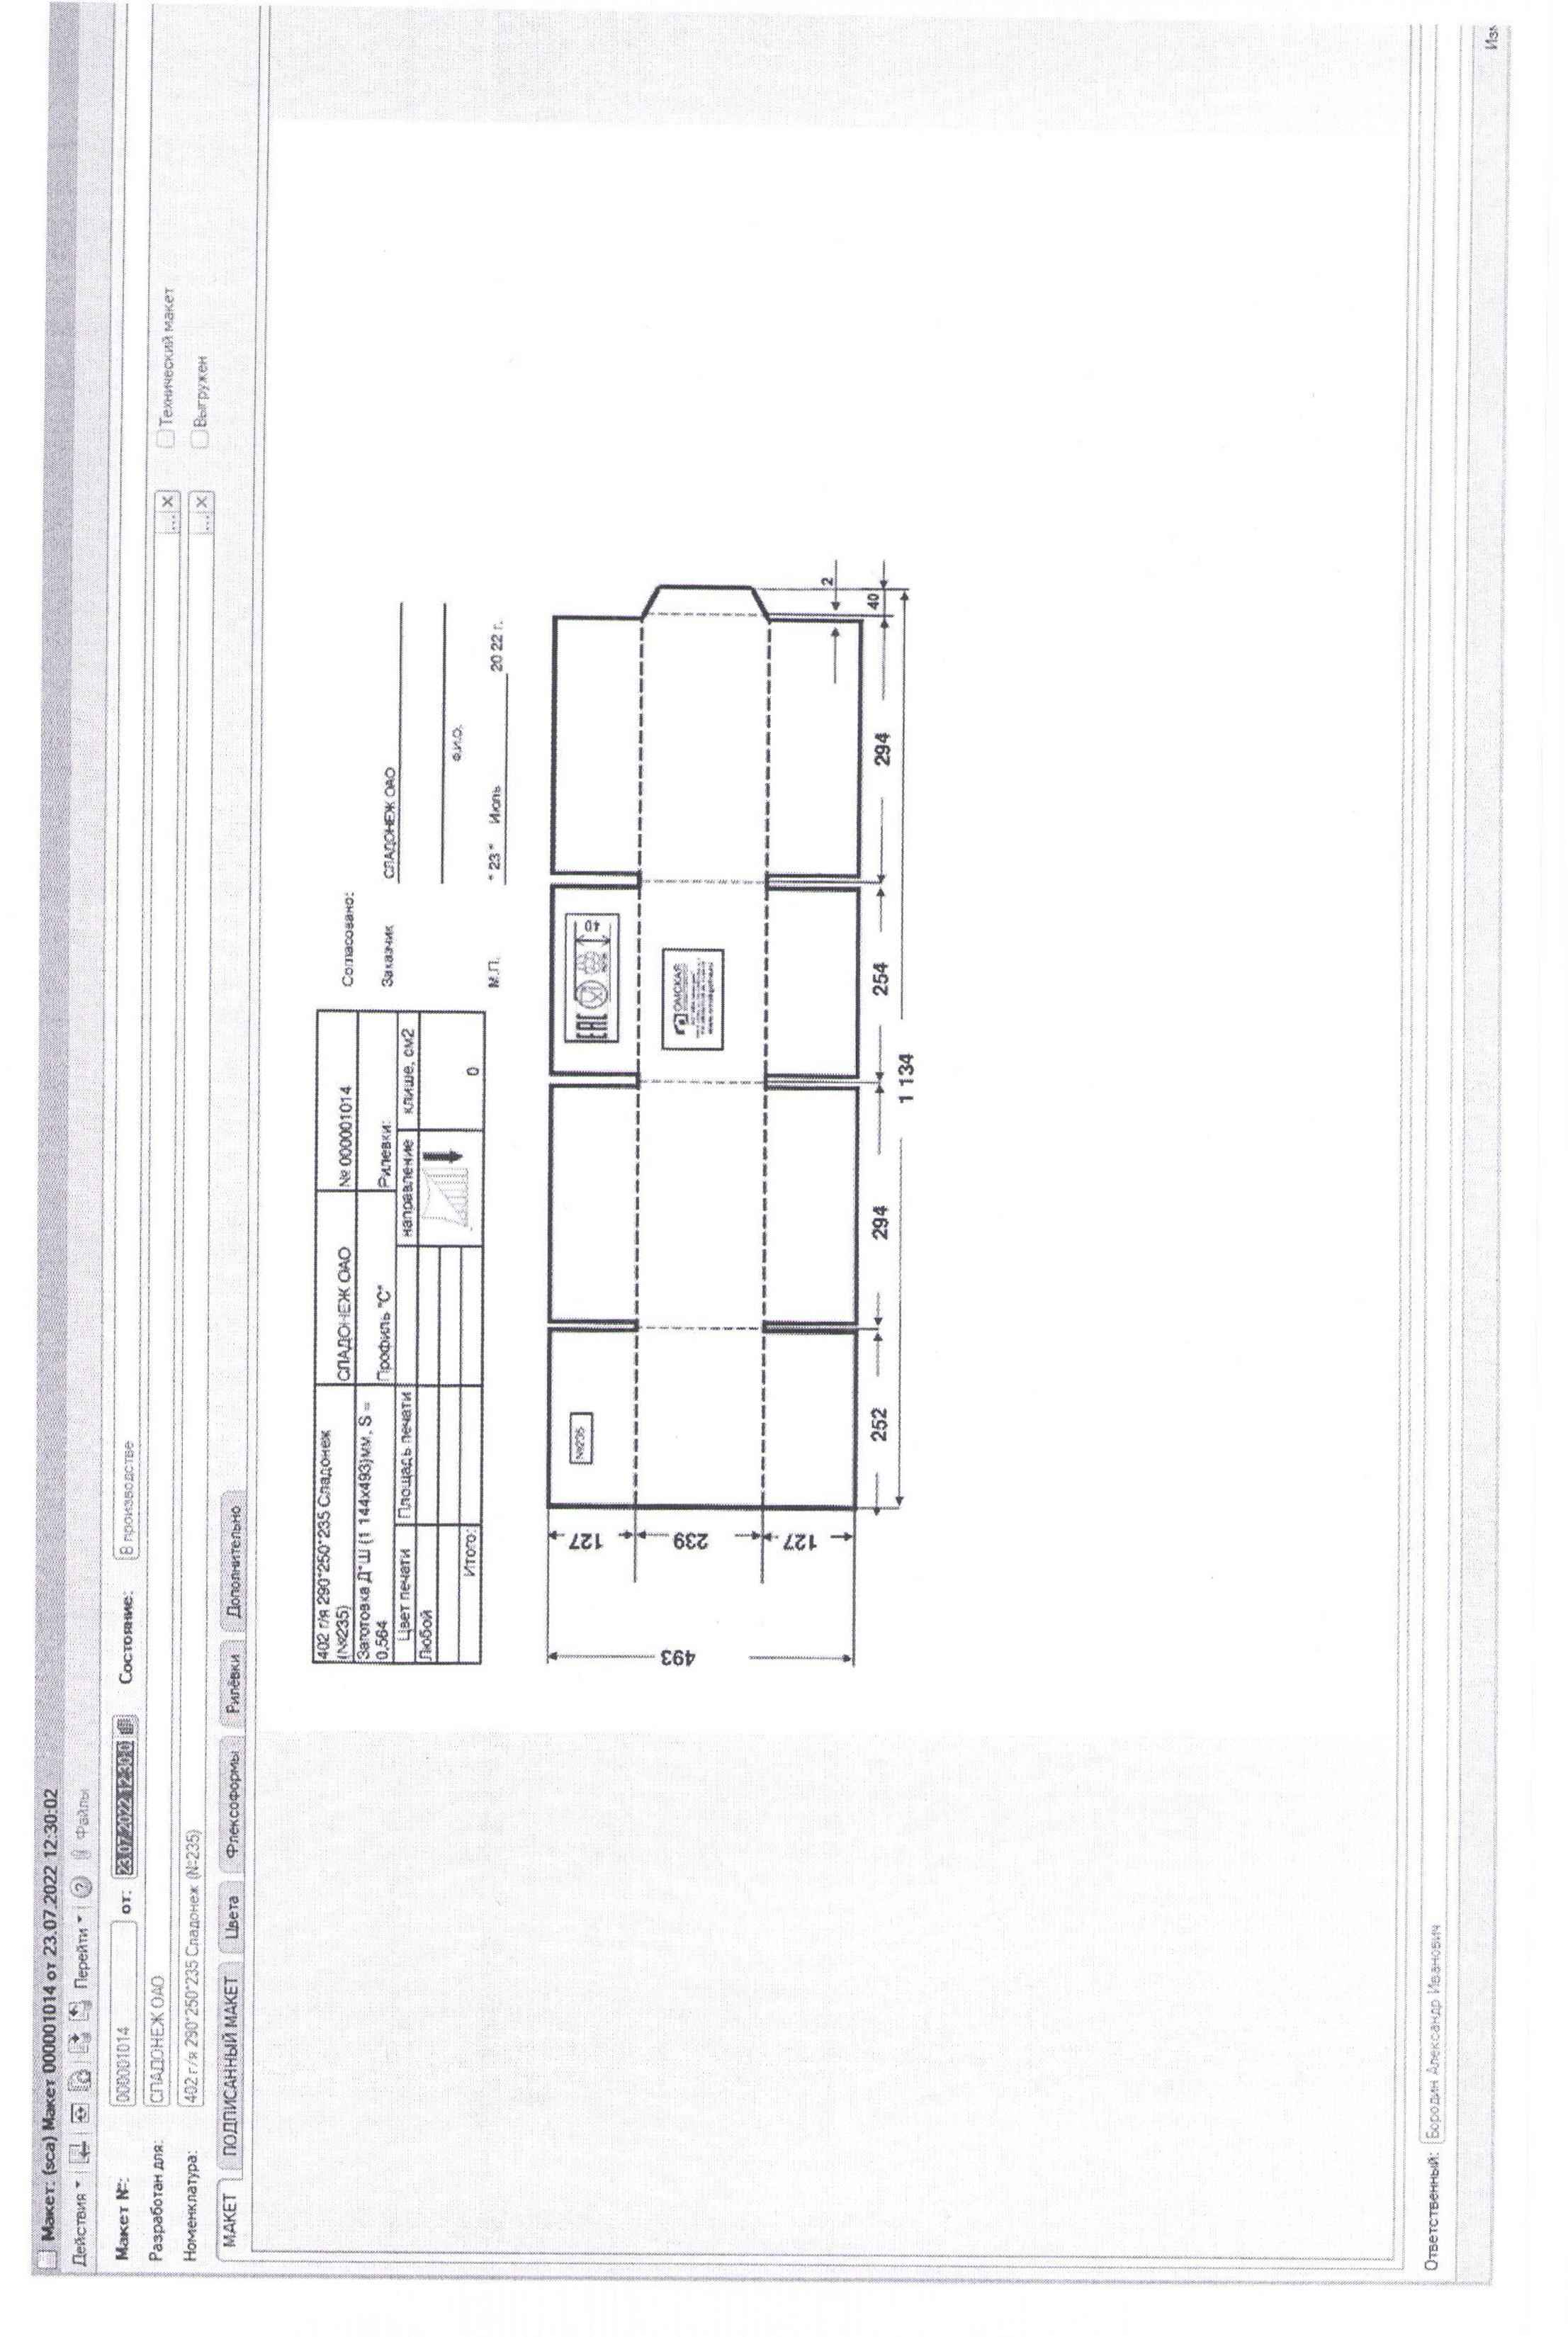
\includegraphics[height=0.94\textheight, width=0.94\textwidth, keepaspectratio]{Pics/d08.jpg}
\end{center}
  \caption{Форма макета техкарты в 1С:УПП}
  \label{pic:d8}
\end{figure}

\begin{figure}
\begin{center}
  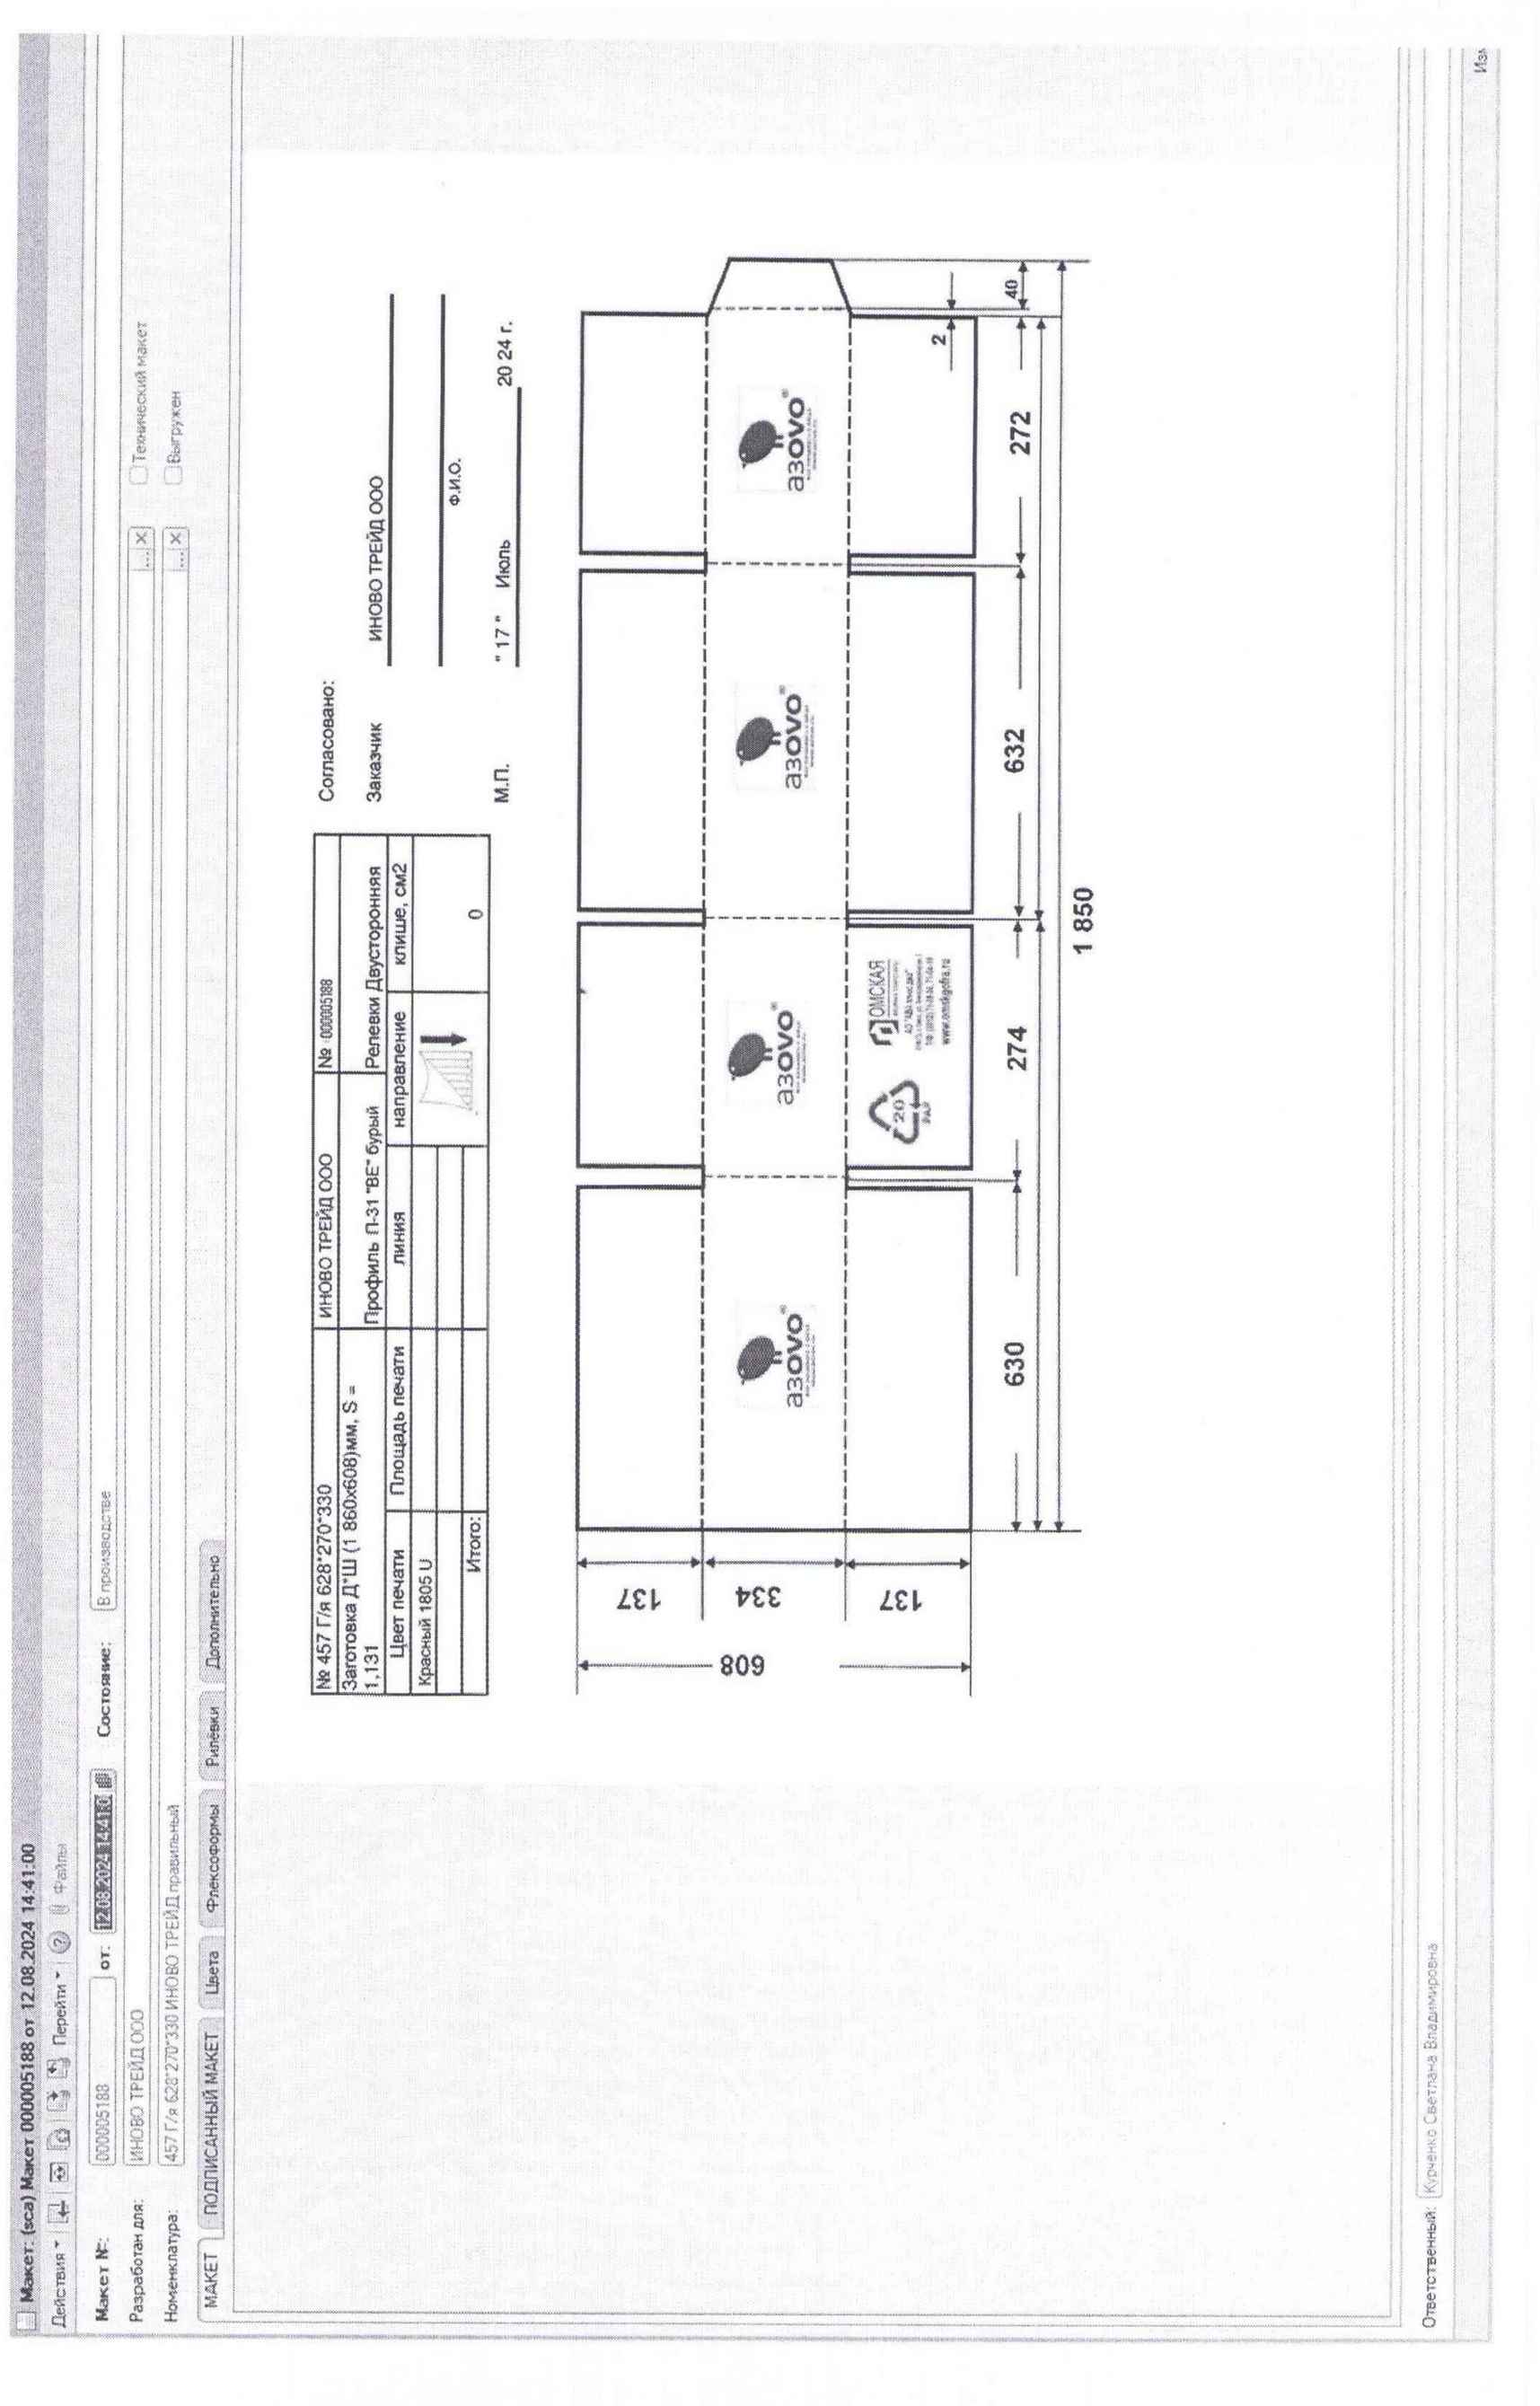
\includegraphics[height=0.94\textheight, width=0.94\textwidth, keepaspectratio]{Pics/d09.jpg}
\end{center}
  \caption{Форма макета на согласование}
  \label{pic:d9}
\end{figure}

\begin{figure}
\begin{center}
  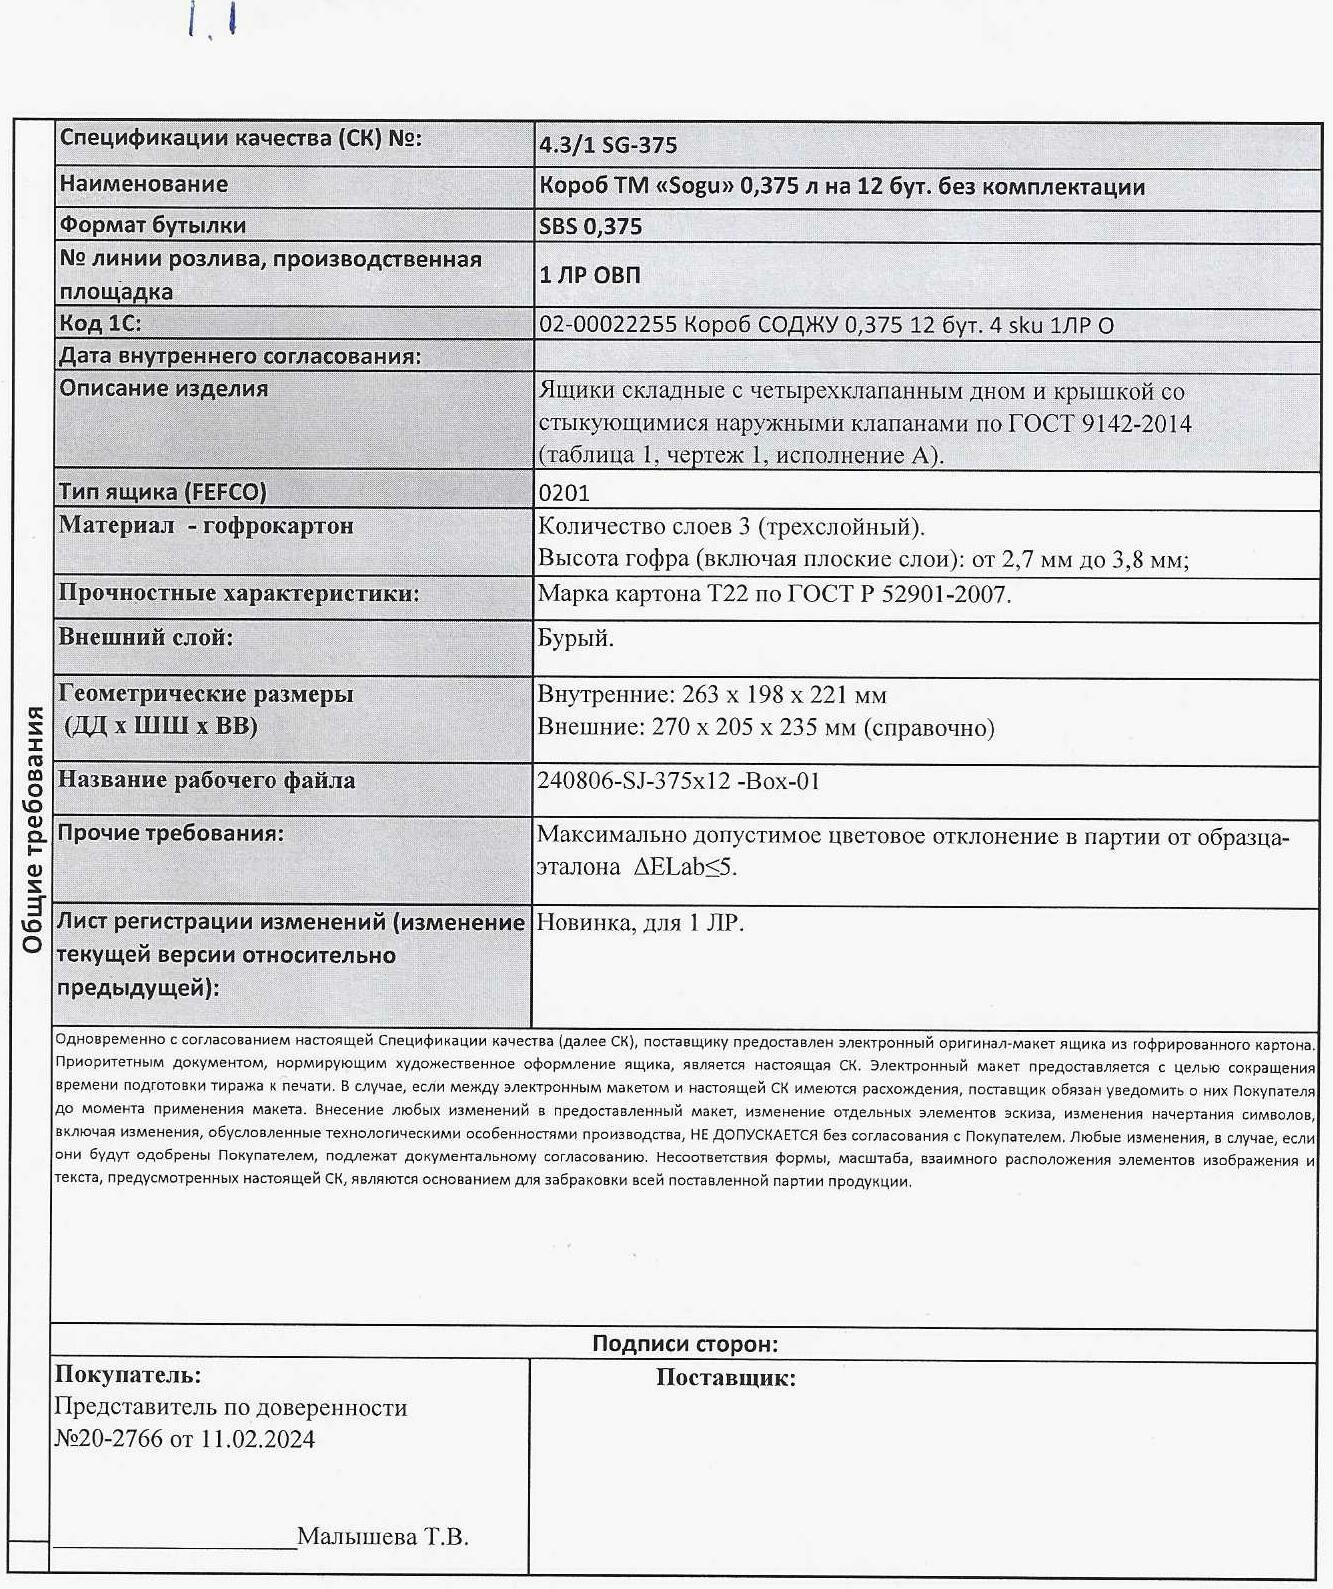
\includegraphics[height=0.94\textheight, width=0.94\textwidth, keepaspectratio]{Pics 1/1.1 спецификация от контрагента_0001.jpg }
\end{center}
  \caption{Спецификация от контрагента}
  \label{pic:1.1 спецификация от контрагента_0001}
\end{figure}

\begin{figure}
\begin{center}
  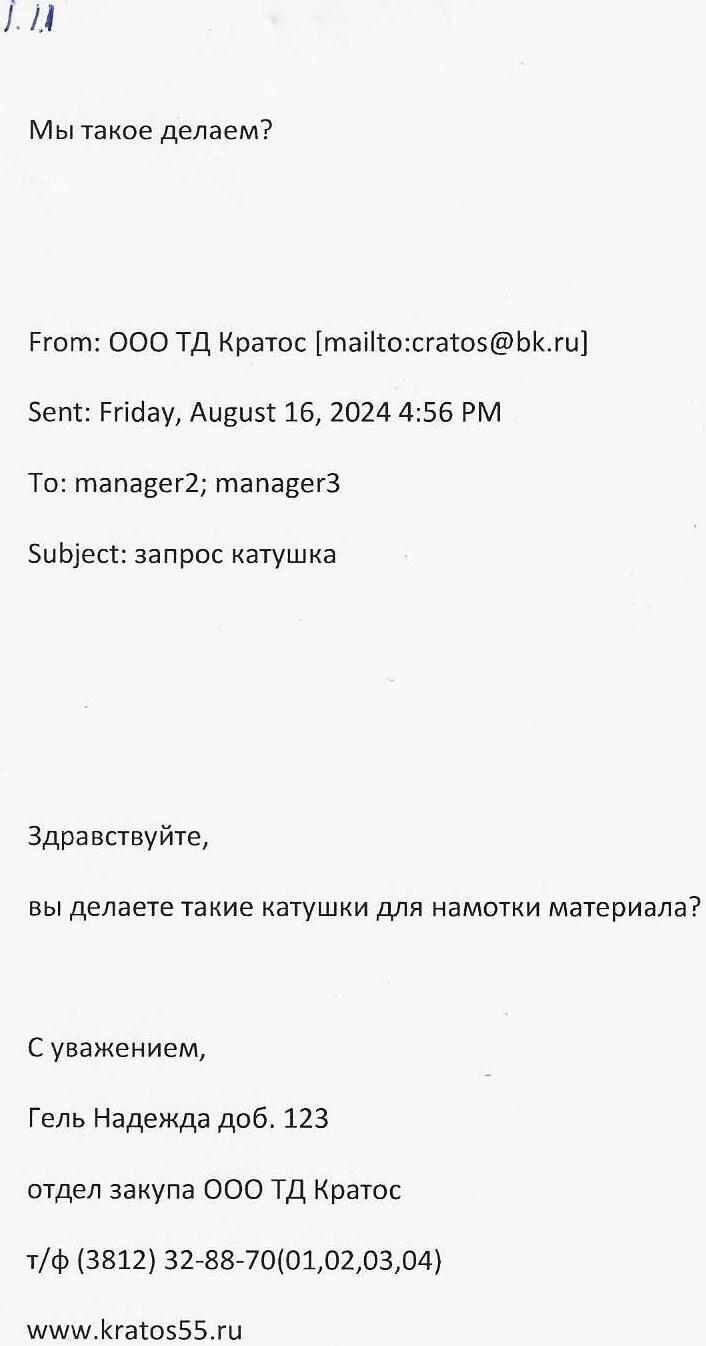
\includegraphics[height=0.94\textheight, width=0.94\textwidth, keepaspectratio]{Pics 1/1.11 запрос от менеджеров к технологу_0001.jpg }
\end{center}
  \caption{Запрос от менеджера к главному технологу}
  \label{pic:1.11 запрос от менеджеров к технологу_0001}
\end{figure}

\begin{figure}
\begin{center}
  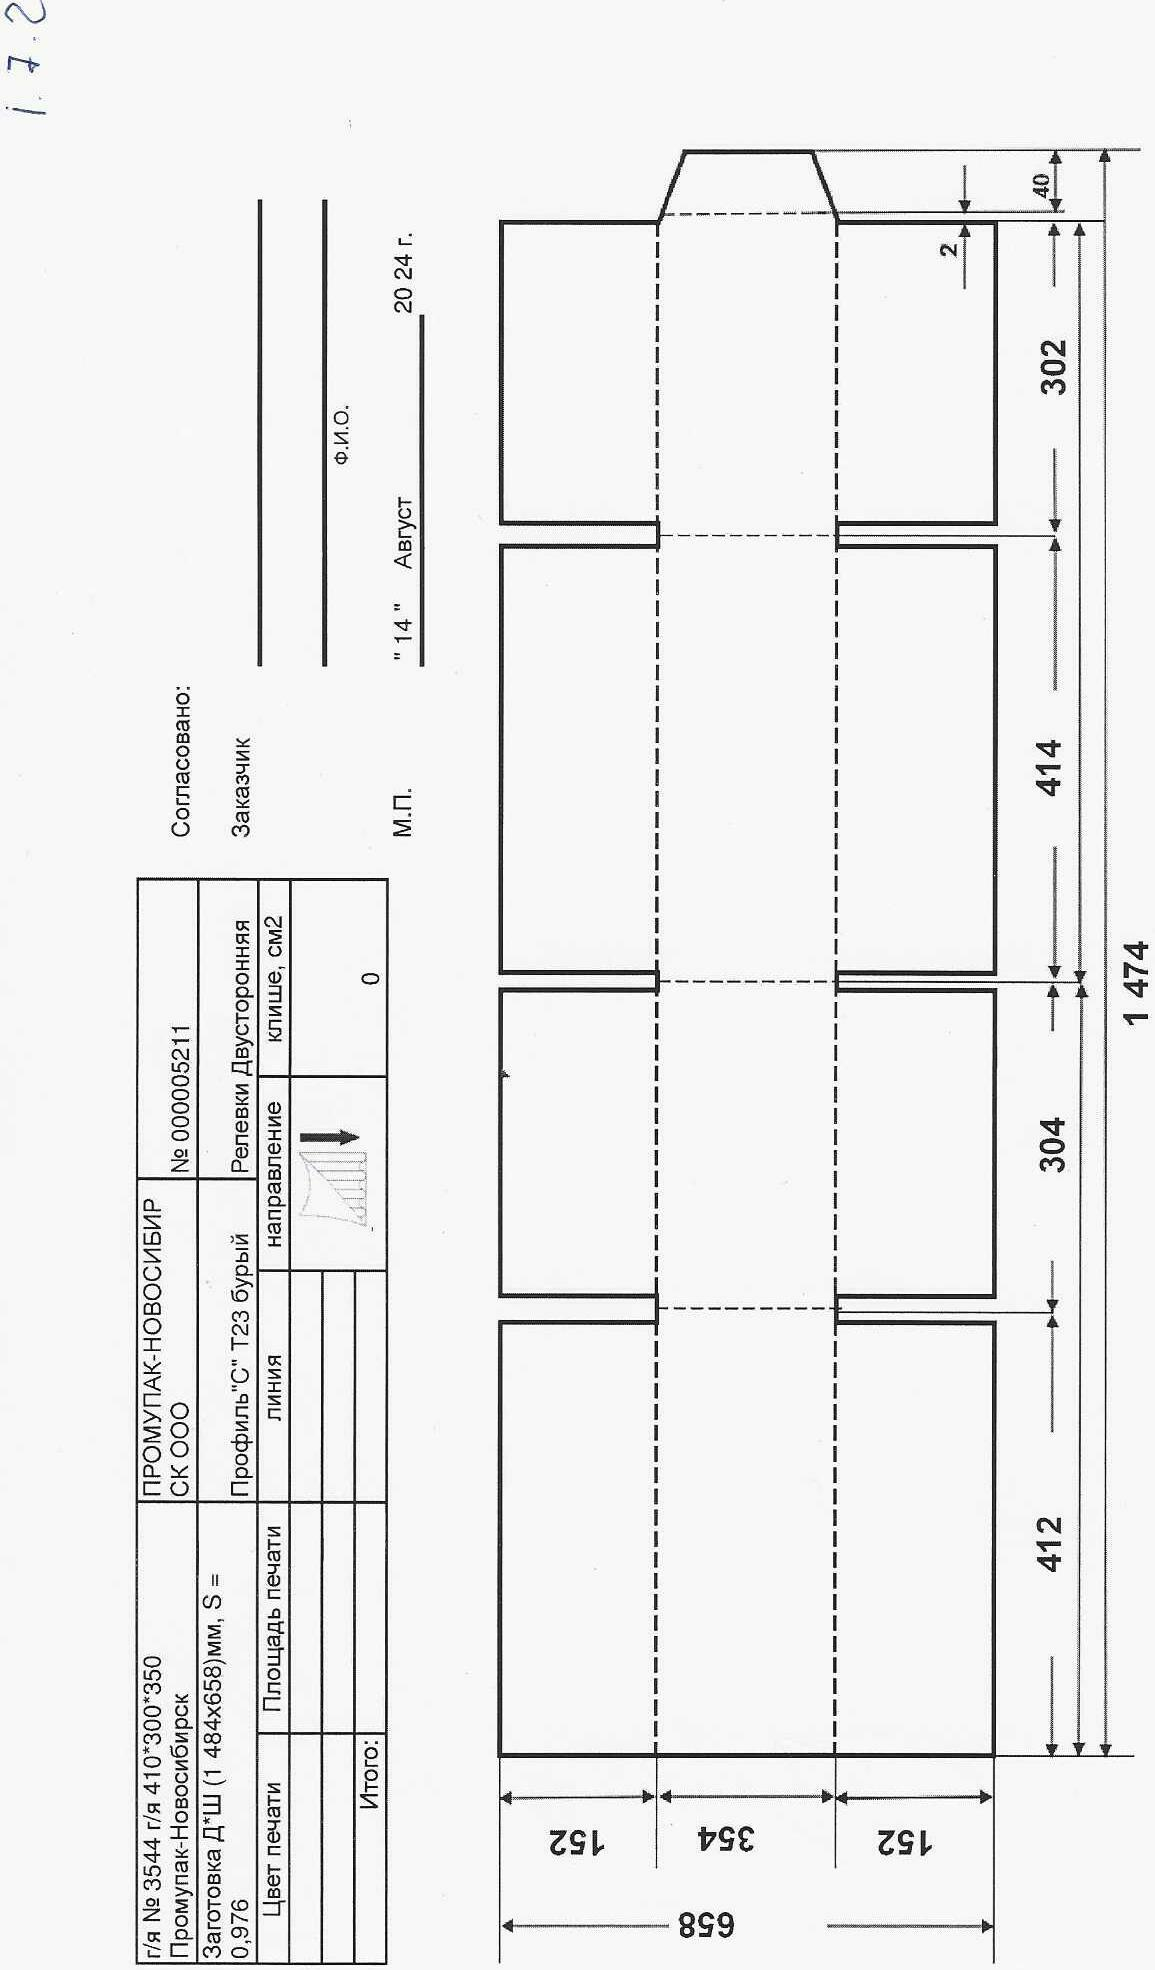
\includegraphics[height=0.94\textheight, width=0.94\textwidth, keepaspectratio]{Pics 1/1.7.2 Макет от менеджера_0001.jpg }
\end{center}
  \caption{Макет созданный менеджером}
  \label{pic:1.7.2 Макет от менеджера_0001}
\end{figure}

\begin{figure}
\begin{center}
  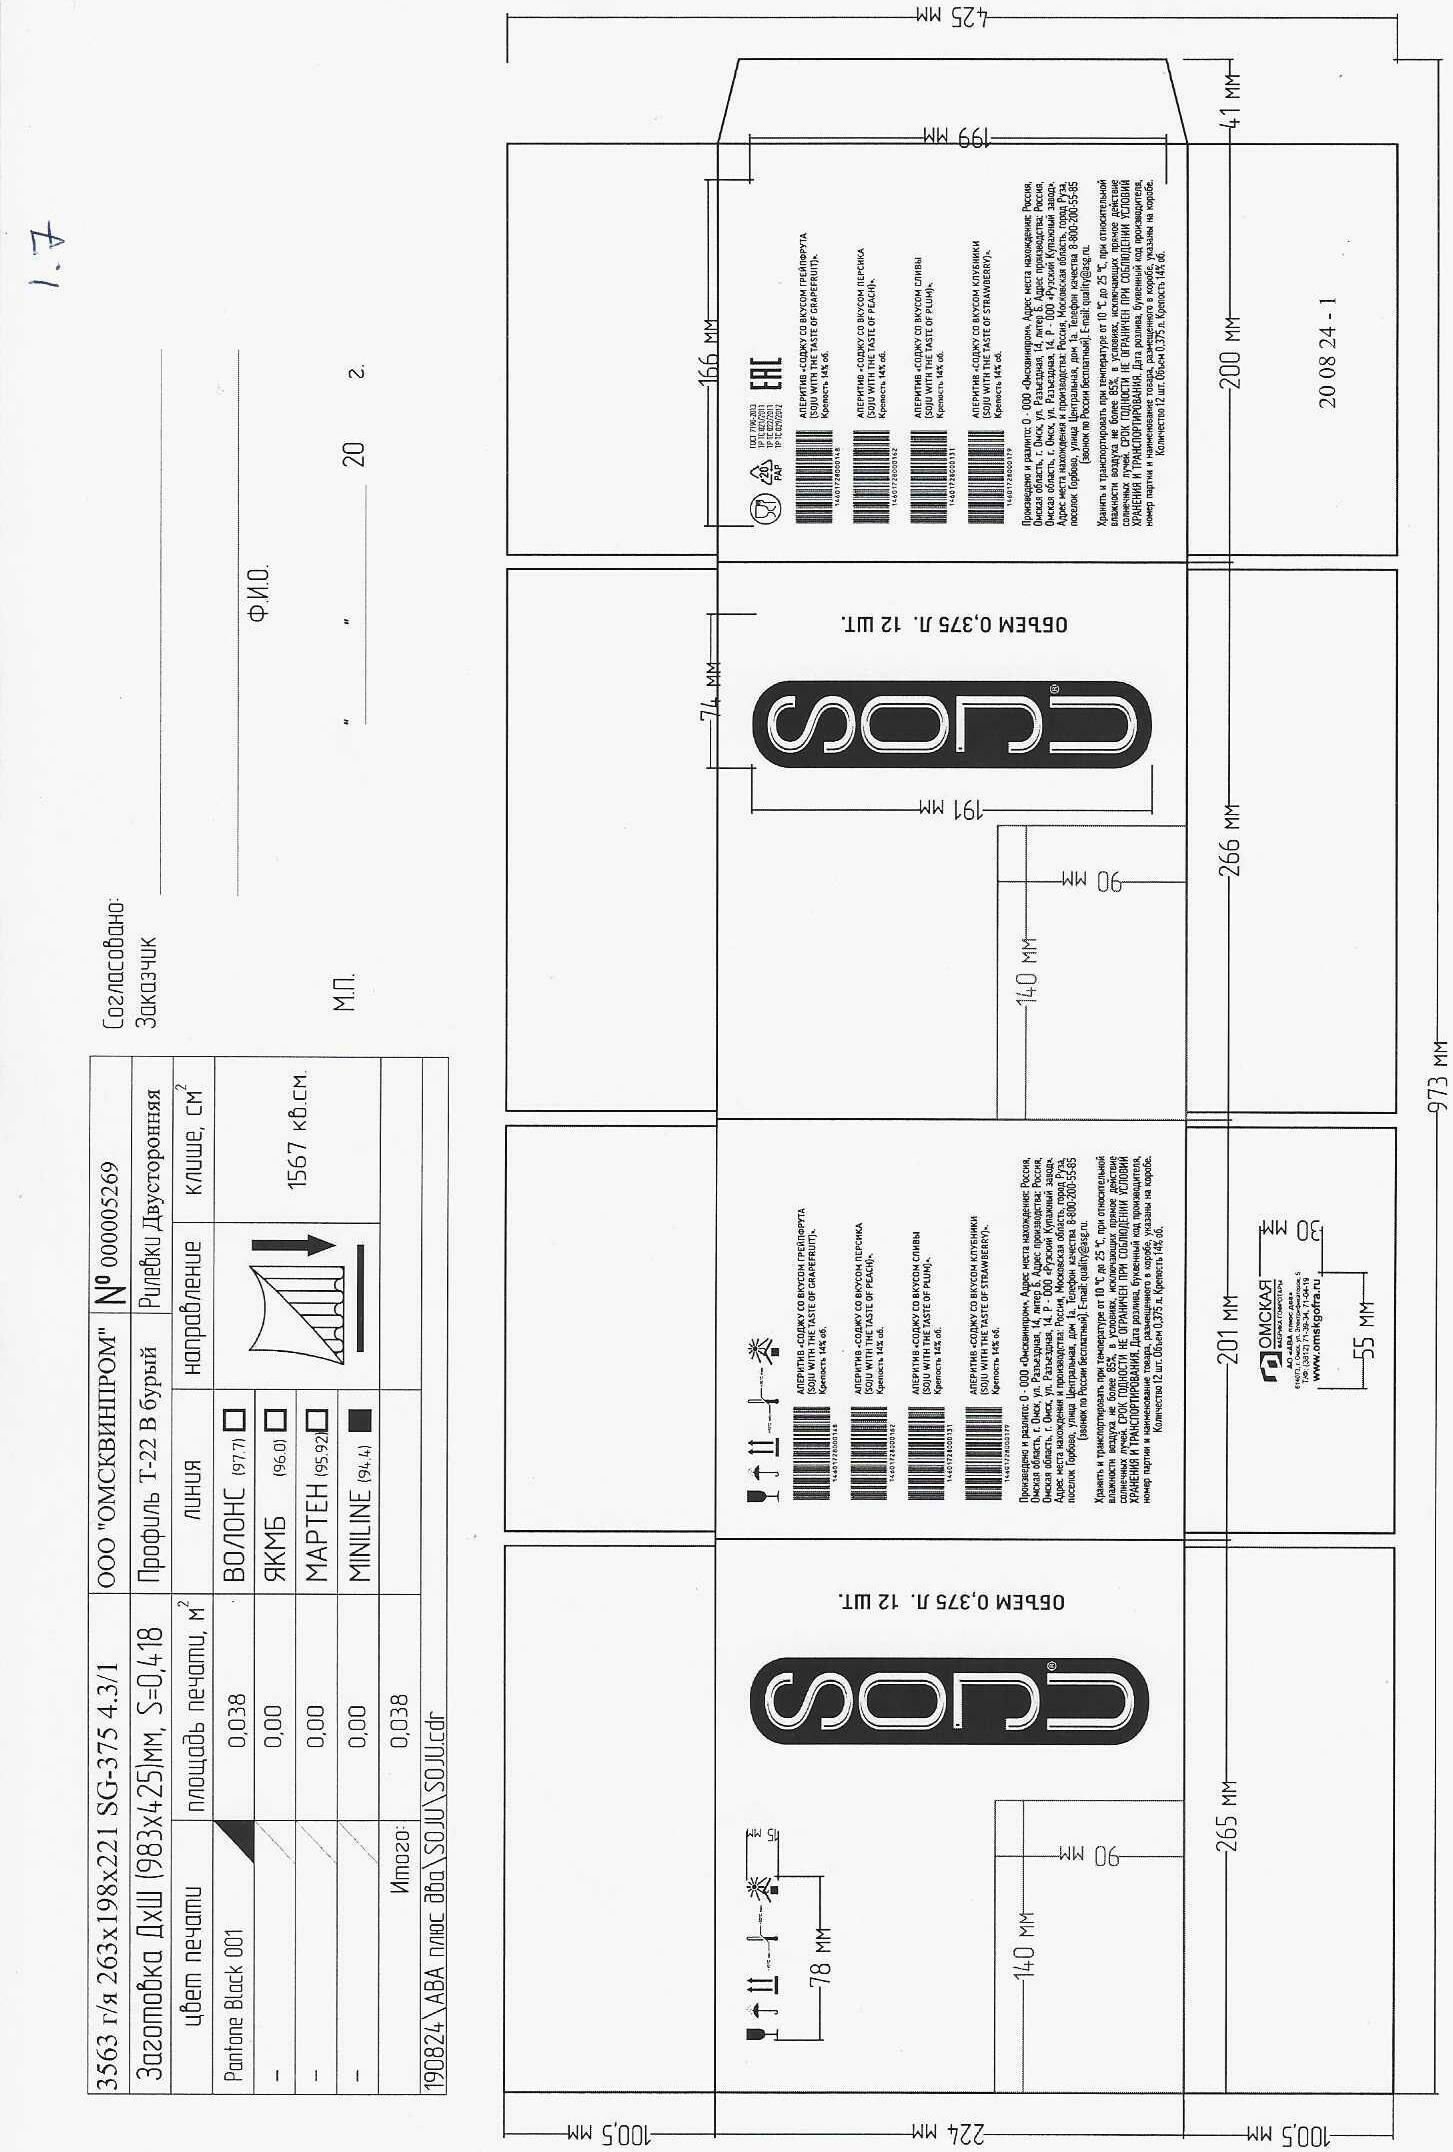
\includegraphics[height=0.94\textheight, width=0.94\textwidth, keepaspectratio]{Pics 1/1.7.1 дизайн от Аверс_0001.jpg }
\end{center}
  \caption{Макет от ООО Аверс}
  \label{pic:1.7.1 дизайн от Аверс_0001}
\end{figure}

\begin{figure}
\begin{center}
  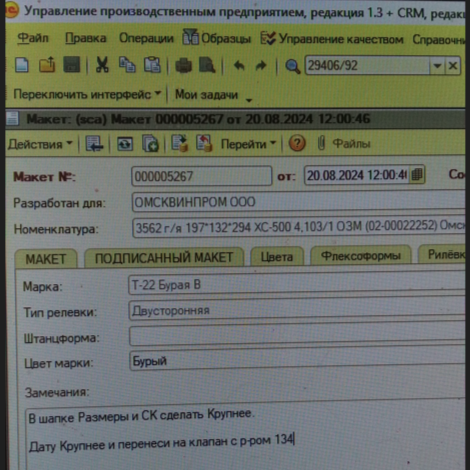
\includegraphics[height=0.94\textheight, width=0.94\textwidth, keepaspectratio]{Pics 1/1 Замечания технолога в ТК.png }
\end{center}
  \caption{Замечания от технолога}
  \label{pic:1 Замечания технолога в ТК}
\end{figure}

\begin{figure}
\begin{center}
  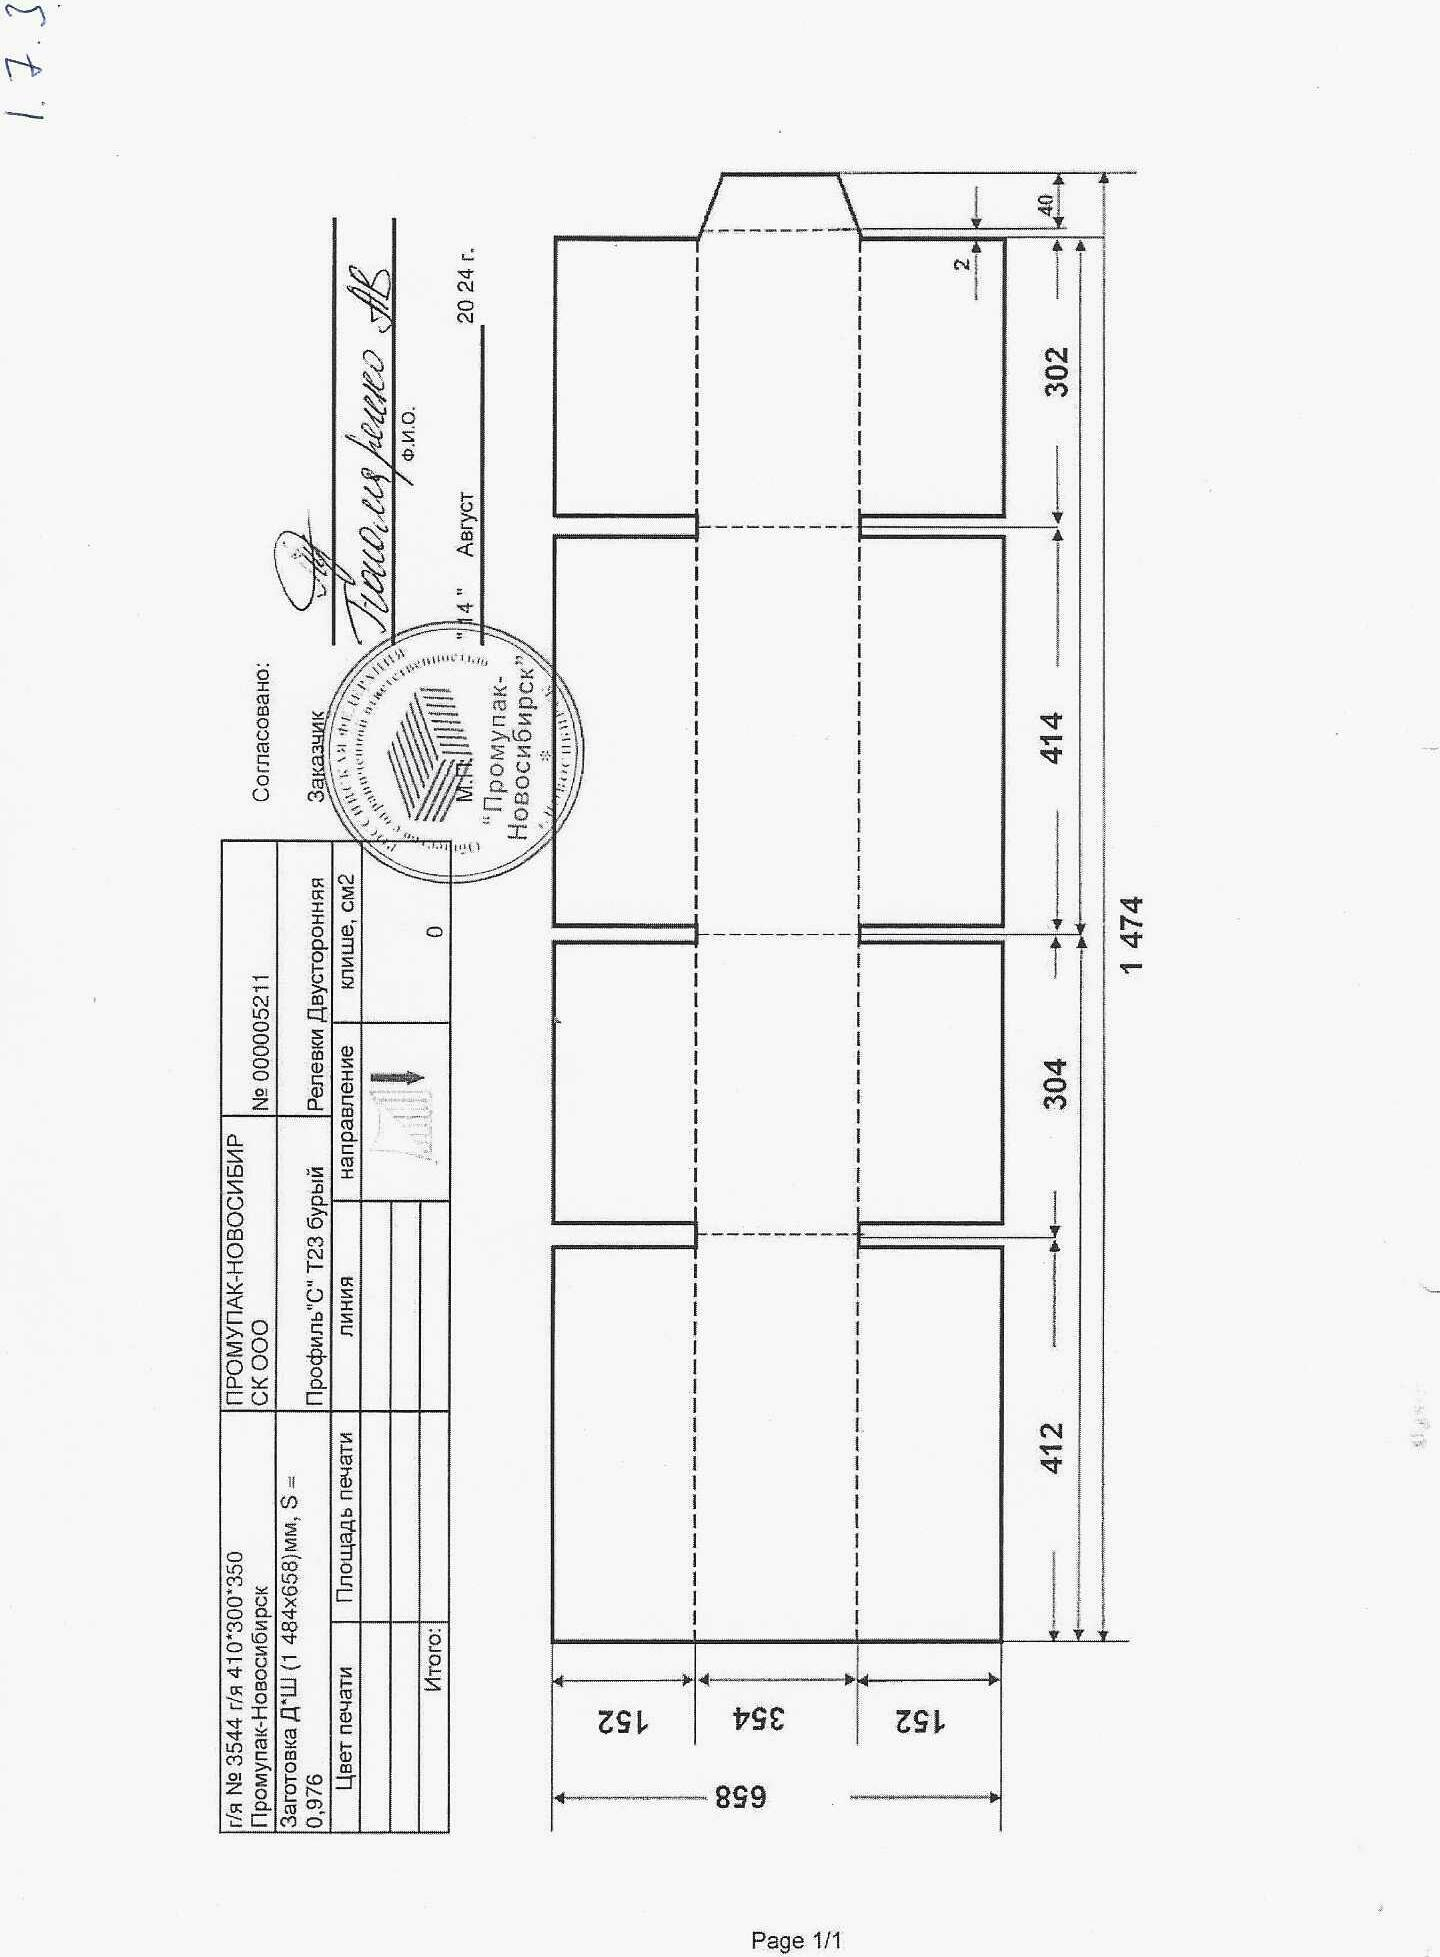
\includegraphics[height=0.94\textheight, width=0.94\textwidth, keepaspectratio]{Pics 1/1.7.3 подписанный макет_0001.jpg }
\end{center}
  \caption{Подписанный макет}
  \label{pic:1.7.3 подписанный макет_0001}
\end{figure}

\begin{figure}
\begin{center}
  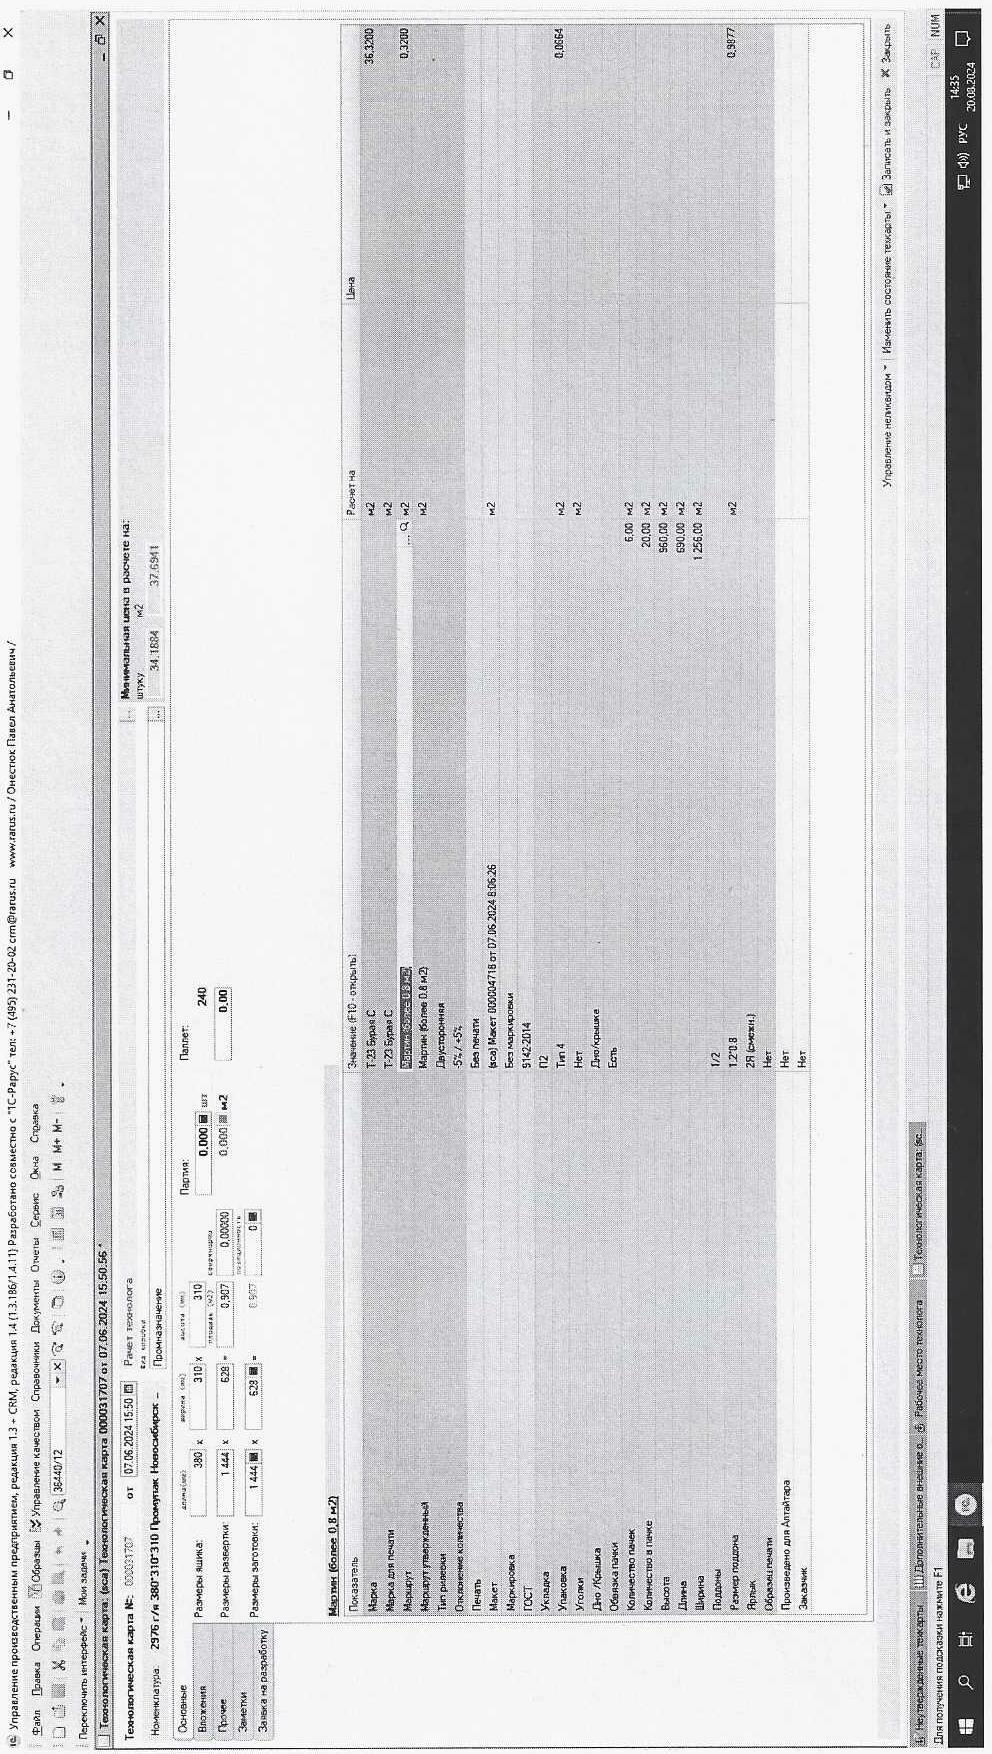
\includegraphics[height=0.94\textheight, width=0.94\textwidth, keepaspectratio]{Pics 1/0 ТК в УПП_0001.jpg }
\end{center}
  \caption{Технологическая карта}
  \label{pic:0 ТК в УПП_0001}
\end{figure}

\begin{figure}
\begin{center}
  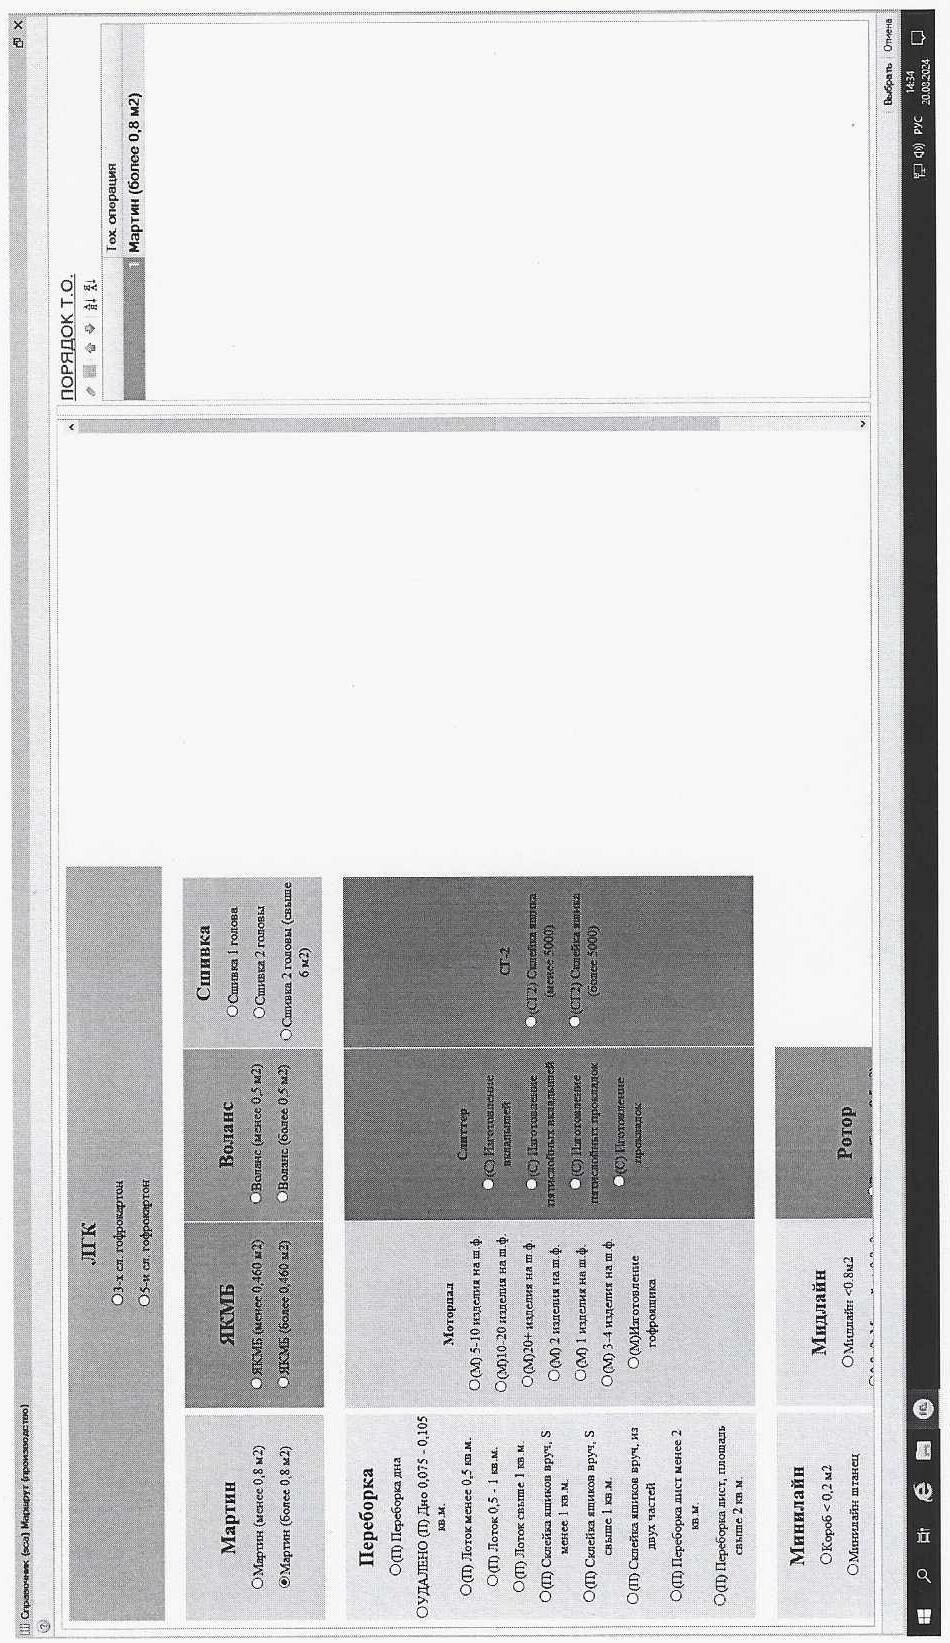
\includegraphics[height=0.94\textheight, width=0.94\textwidth, keepaspectratio]{Pics 1/0 определение маршрута_0001.jpg}
\end{center}
  \caption{Определение маршрута в системе 1С:УПП}
  \label{pic:0 определение маршрута_0001}
\end{figure}

\begin{figure}
\begin{center}
  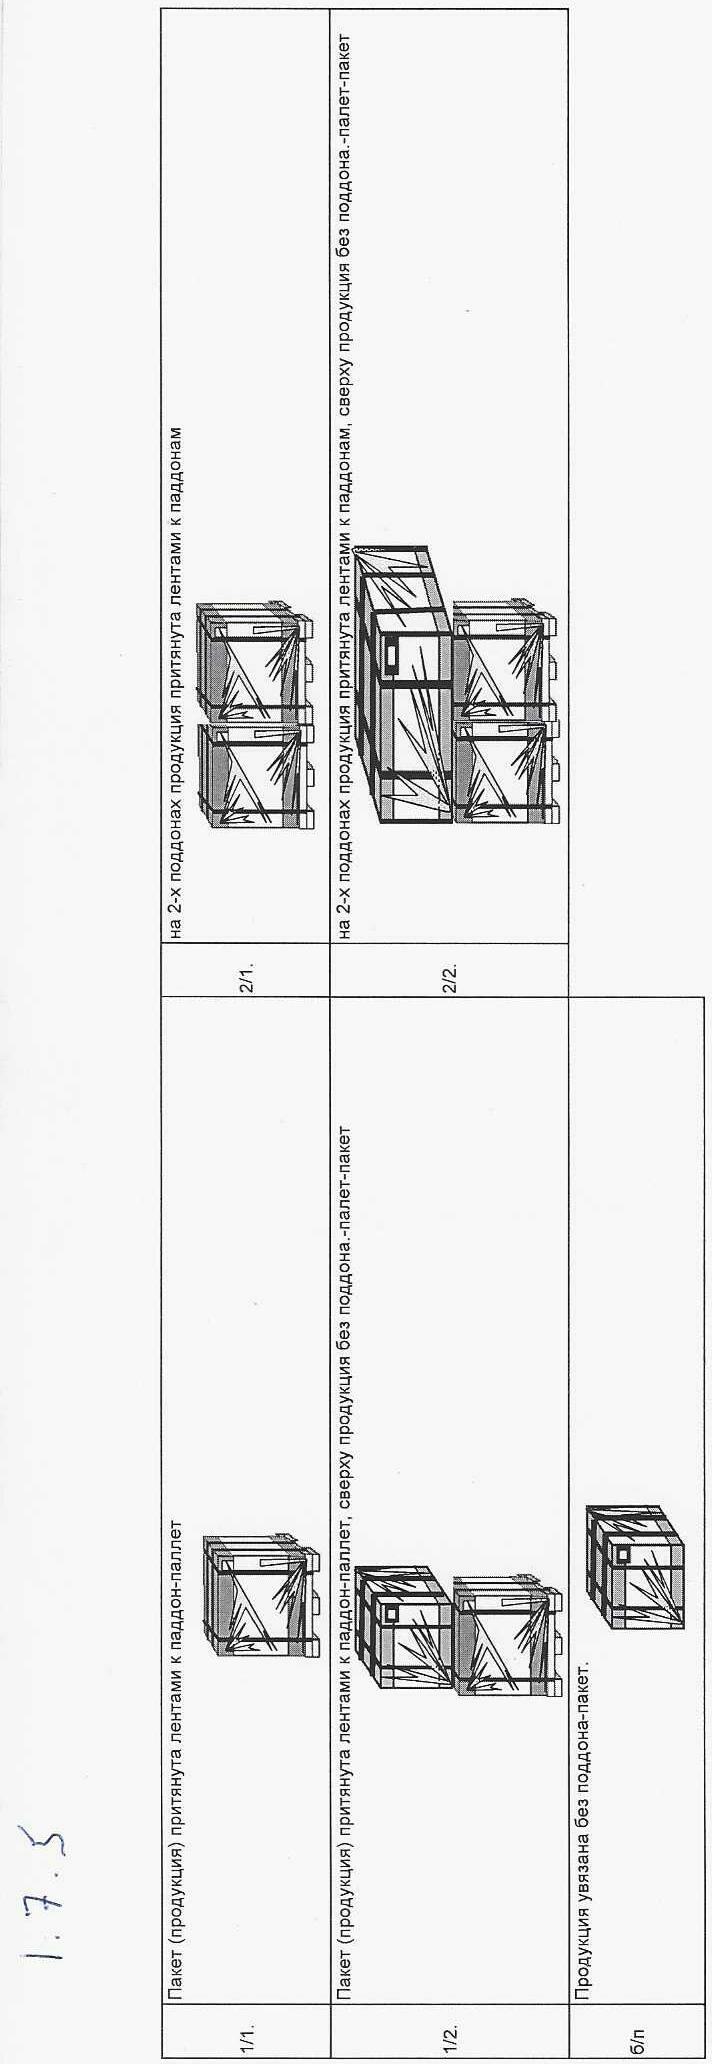
\includegraphics[height=0.94\textheight, width=0.94\textwidth, keepaspectratio]{Pics 1/1.7.5 схемы упаковки_0001.jpg}
\end{center}
  \caption{Схемы упаковки}
  \label{pic:1.7.5 схемы упаковки_0001}
\end{figure}

\begin{figure}
\begin{center}
  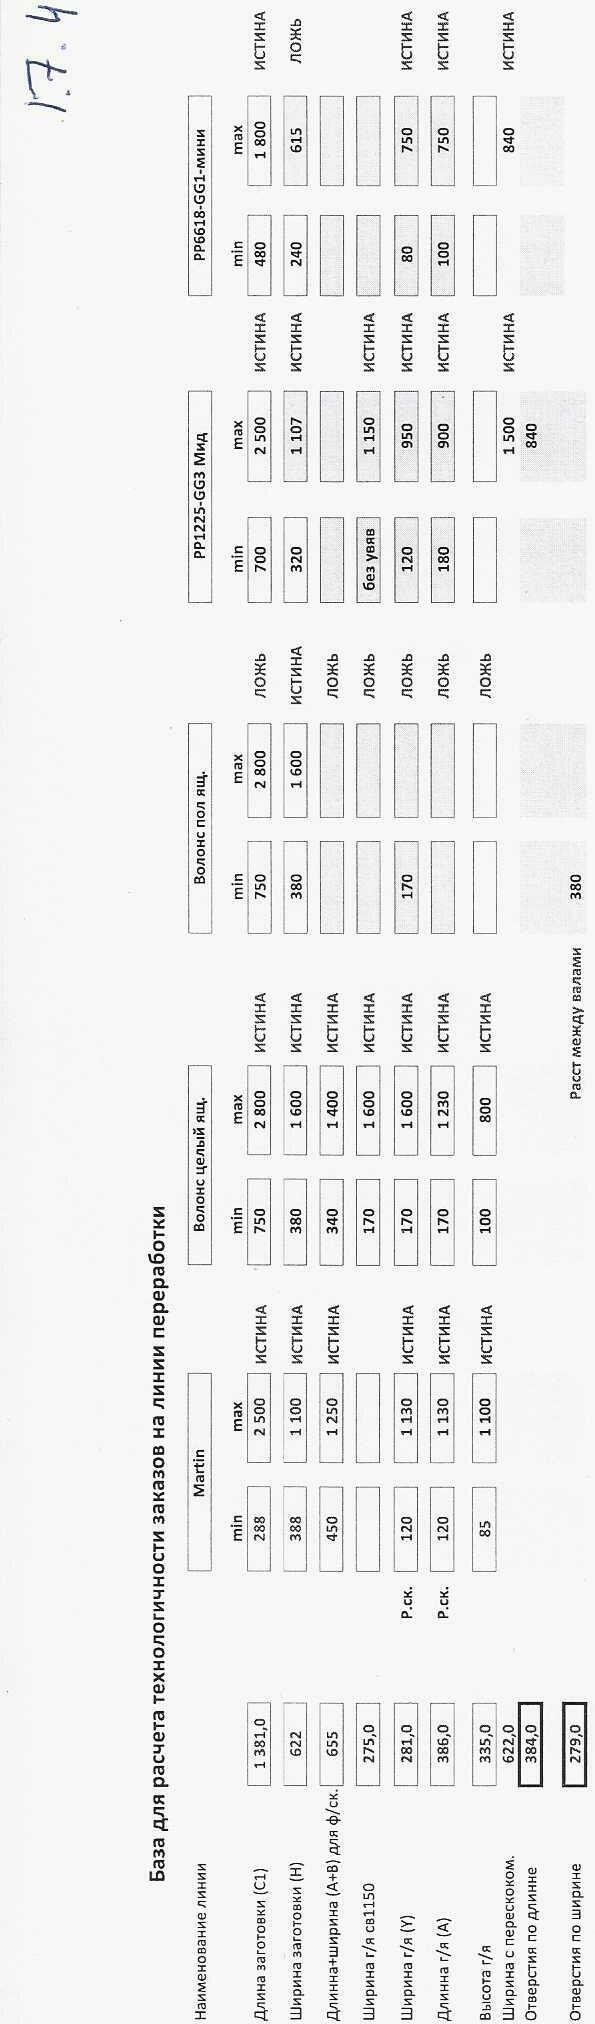
\includegraphics[height=0.94\textheight, width=0.94\textwidth, keepaspectratio]{Pics 1/1.7.4 справочник для маршрутов_0001.jpg}
\end{center}
  \caption{Справочник размеров}
  \label{pic:1.7.4 справочник для маршрутов_0001}
\end{figure}

\begin{figure}
\begin{center}
  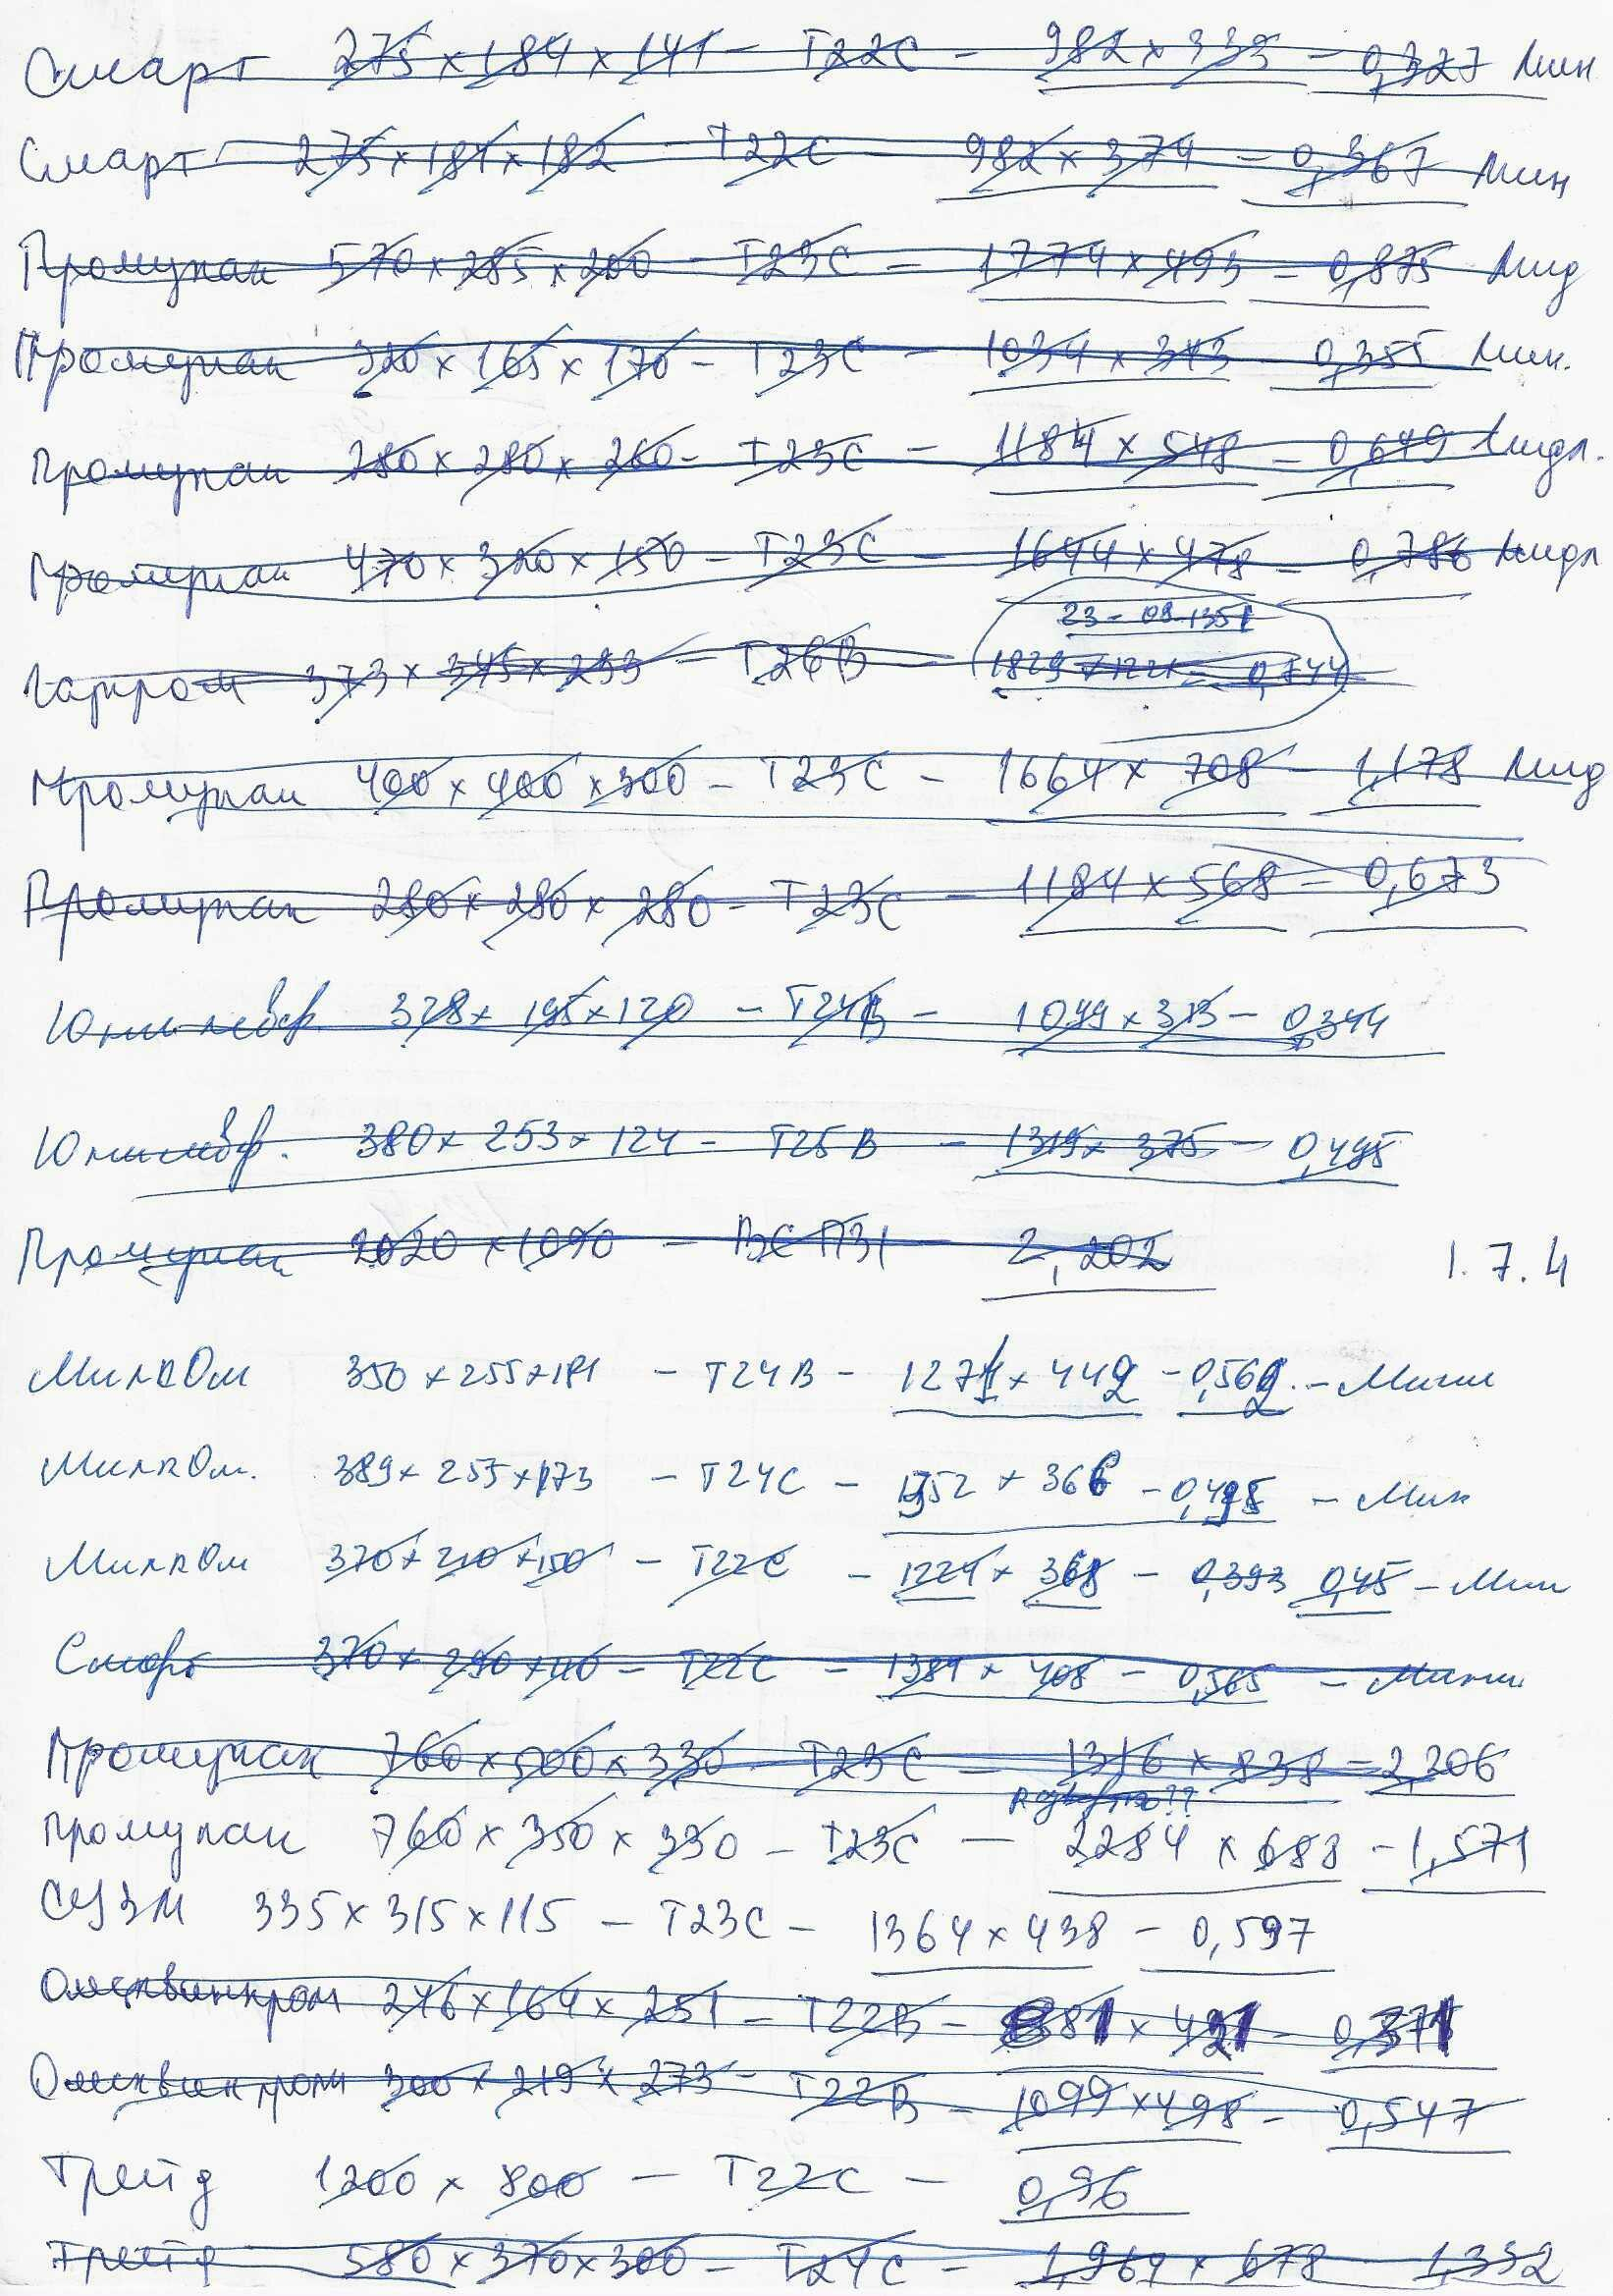
\includegraphics[height=0.94\textheight, width=0.94\textwidth, keepaspectratio]{Pics 1/1.7.4 список проверенных ТК_0001.jpg}
\end{center}
  \caption{Список проверенных ТК}
  \label{pic:1.7.4 список проверенных ТК_0001}
\end{figure}


%Менеджер в системе 1С CRM заполняет опросный лист (1). У инженера загорается задача в системе 1С CRM (ф1), при дальнейшей работе с этим опросным листом меняются автоматически статусы (ф2).

%Для 4-х клапанного короба по опросному листу инженер смотрит применение коробки и присваивает ТУ, ТУ 068 – пищевой короб, ТУ 069- промышленный короб (ф3). Далее смотрят размеры, был ли короб ранее с такими размерами, если был, то ищут на сервере в таблице EXCEL (ф4) присвоенный ему номер, если не было ранее такого короба, то ему присваивают номер. Далее в EXCEL шаблоне создают ТК (ф5). В 1С CRM автоматически формируется артикул, который состоит из ТУ, размеров короба и варианта исполнения. (ф4а), (3,4).

%Для проверки технологичности и возможности изготовления короба, применяют расчетный шаблон в EXCEL (ф5а), если проверку не прошло, но у инженера есть предположения, что данный короб могут изготовить, то отсылают на согласование на производство.

%Иногда менеджер может принести образец от клиента и тогда инженер производит замеры и подбирают нужный короб. Для замеров решетки, могут принести пустые бутылки.
%Если есть комплектующие, то в опросном листе 1С CRM будет указано к коробу есть решетка или решетка к коробу №….

%На сложную высечку могут дать ссылку в каталоге FEFCO или принести чертеж от клиента. При обращении клиента через личный кабинет, и отсутствии чертежей, общение с клиентом может осуществлять инженер через личный кабинет, предлагая различные варианты. Могут прислать фото короба (ф6).

%Сложную высечку чертят в программе AUTOCADE. (ф 6а). После разработки чертежа в 1С CRM в опросном листе, в графе ОПЗ присваивают номер чертежа (ф 7а). Переводят чертеж в PDF и прикрепляют в опросный лист для согласования. После согласования с клиентом, менеджер в программе 1С CRM запускает процесс заказа штампа. Служебная записка проходит согласование разных служб, в ней указывается доходность этого короба, для принятия решения руководителю. (ф 10). После согласования в AUTOCADE разрабатывают чертеж заготовки и раскладку на штампе (ф 11,12), присваивают им номера чертежей. Указывают направление гофры по сторонам (длинна или ширина) (ф 13). Далее присваивают номер ящика, если он был размерным, находят по номер по размеру. (ф 7,8). Все файлы прикрепляют в опросном листе в графе «файл» (ф 9, 14), затем отправляют на согласование в производство (ф 15). 

%После согласования производства, в EXCELE таблице (ф 16) на сервере по линиям создают папку с номером ящика, куда вкладывают все чертежи для заказа штампа. Если штамп заказывают за счет клиента, то после оплаты заказывают штамп. Папку с чертежами отправляют в Растр технологии или Лазер Пак. (ф 16а). Изготовители присваивают номер заказа и перечерчивают чертеж штампа с указанием всех параметров (ф 17а), отправляют на согласование. Далее инженер согласовывает в программе 1С CRM (ф 17б) и отправляет назад согласованный чертеж штампа. Ожидают счет на оплату (ф 17в) и при его поступлении вкладывают в файл в папку снизу опросного листа, не для видимости клиента (ф 17г). 

%О приходе штампа сообщает технолог из цеха или отслеживают сами. После прихода штампа заполняют таблицу EXCEL на сервере (ф 18а) и в папке паспорта (ф 19) создают паспорт на штамп (ф 20). После заполнения все чертежи отправляют в цех технологам, где они заполняют «эксплуатацию штампа».

% При разработке макета печати используют файлы, вложенные в опросном листе (ф 21), реже подбирают логотипы из интернета или обрисовывают в CorelDRAW, масштабируют по коробу. Дизайн не разрабатывают. Рисунки от клиентов необходимы в векторном файле, если рисунок пришел не в соответствующем разрешении или более 3-х цветов, то отправляют на корректировку клиенту. 
 
% Если все данные подходят, то из таблицы EXCEL на сервере (ф 22) берут порядковый номер и в программе 1С CRM занимают место с этим номером. 
 
% Эскиза печати загружают в опросный лист в 1С CRM и отправляют на согласование в производство. (ф 23, 23а). После согласования производством, эскизы отправляют на согласование с клиентом, в личном кабинете или через менеджера.
 
% Согласованные эскизы печати выкладывают на сервер в папку CDR (ф 24а), оттуда инженер берет эскизы и накладывает на ящик при создании ТК.
 
% По согласованию с клиентом, на все короба ставят номерной штамп. На этом штампе меняют площадь и номер короба. (ф 24).
 
% Затем менеджер создает заявку на заказ клише. Если в заявке стоит галочка «счет на клише» - это означает, что это клише необходимо заказать, если такой галочки нет, значит клише есть на производстве. (ф 25а).
 
% После согласований, приходит задача дизайнеру на заказ клише в 1С CRM. Дизайнер готовит пакет чертежей и нужную документацию (ф 25, 25б). Если короб сложной высечки, то прикладывают чертёж заготовки. Создают заявку (ф 26) и весь пакет документов отправляют по электронной почте в РЕПРОПАРК. После обработки РЕПРОПАРК высылает макет на согласование и счет.
 
% На ГЦ2 в основном заказывают полимеры, т.к. есть свой отдел по подготовки оснастки, где монтажисты наклеивают полимеры на фартук, на ГЦ1 такой отдел отсутствует и клише, адресованные на эту площадку, заказывают уже готовым комплектом.
 
% Далее делается чертеж монтажа полимеров, который отправляют по электронной почте монтажистам. Все согласованные чертежи выкладывают на сервер (ф 26а).
 
% После заказа оснастки, менеджер по работе с поставщиками отдела подготовки производства, отслеживает приход, о котором сообщат по электронной почте или в таблице.
 
% Перед приходом оснастки, распечатывают счет (ф 27а), заносят в 1С участок вырубных форм и дублируют в EXCEL таблице на сервере (ф 27). При поступлении оснастки заносят приход в 1С участок вырубных форм, а в EXCEL таблицу вносят УПД.
 
% Списание оснастки происходит по акту от производства (ф 28).
 
% Один раз в пол года проводят инвентаризацию оснастки. В таблицу EXCEL вносят оснастку, не использованную за последние два года и отправляют менеджерам, для пометки о ее дальнейшей судьбе – отдать клиенту, оставить или утилизировать. 
 
% При разработке ТК на 4-х клапанный короб, карта упаковки разрабатывается сразу в EXCEL. При сложной высечки, карта упаковки разрабатывается позже. После прикрепления чертежа в опросный лист, поступает задача инженеру на разработку упаковки. Инженер заполняет в 1С CRM габариты пачки (ф 29) и программа автоматически рассчитывает укладку на паллет, высоту паллеты и т.д. (ф 30). Номер карты упаковки формируется автоматически.
 
% После инженер создает заявку на номенклатуру, она создается в 1С участок вырубных форм отделом планирования ГОЛОВАНОВО. В 1С участок вырубных форм карта упаковки загружается спецификацией. 
 
% При планировании в отделе планирования видят поступление нового заказа без ТК, заходят в 1C CRM APM технологическая документация, по номенклатуре или артикулу находят необходимую ТК и подгружают ее (ф 31), также руками переносят в PC Topp. 
 
% Общее количество ТК не известно, за последний год было разработано 5867 ТК.
%Штампов более 1200, клише более 2000 штук.


%Менеджер получает запрос на разработку нового изделия только по почте от клиента.

%Заявка на изготовление нового изделия поступает от менеджера к дизайнеру в журнале MS Exсel.
%При отсутствии на заявке артикула отдел учёта создаёт новое здание. Для существующих изделий присвоен артикул, который менеджер указывает в комментарии в заявке .

%Менеджер формирует заявку (рис. \ref{pic:pic_d7}), высылает в отдел учета.  Отдел учёта создает номенклатуру в программе 1С: 7.7. Бухгалтерия по требованиям менеджера (рис. \ref{pic:pic_d7}). При отсутствии номенклатуры отдел учета создает новую номенклатуру в системе 1С: 7.7. Бухгалтерия и заявку в справочнике заявок. 

%Отдел учета в системе 1С: 7.7. Бухгалтерия и в таблице MS Excel указывает категорию цены, которая зависит от периода.

% При разработке сложного изделия с печатью менеджер формирует заявку дизайнеру на изготовление клише. Дизайнер разрабатывает макет клише в программе CorelDraw.  Готовый макет дизайнер высылает менеджеру в формате JPEG. 
% Менеджер согласовывают с клиентом макет печати технологической карты  изделия.

%Менеджер выставляет счёт покупателю на изготовление клише при необходимости. Дизайнер заказывает  изготовления печатной формы у стороннего производителя (см. процесс ''Учет оснастки \ref{bp:rigging}). 

% При разработке нового изделия сложной высечки менеджер создает задание на разработку штанцформы дизайнеру на разработку и чертёж от клиента  в электронном виде. Форма заявки на разработку нового изделия пересылается менеджером по электронной почте или Skype дизайнеру Московский офис. 
%Дизайнер в свою очередь передает задание конструкторское бюро конструктору для разработки штанцформы \ref{pic:pic_a36}.  Конструктор разрабатывает в программе AutoCAD  макет штанцевальной формы.  После согласования макет конструктор распечатывает  чертеж на большем принтер-плоттере в масштабе 1:1, прилагает чертёж на формате А4 и передает в отдел штампов.

%Менеджер контролирует изготовление макета штанцевальной формы. 
%Готовый макет конструктор высылает дизайнеру, дизайнер проверяет макет и высылает менеджеру (рис. \ref{pic:pic_d16.1}). 
%Менеджер согласует конструкцию изделия с покупателем эскиз \ref{pic:pic_a3}. 
%Стоимость штампа почти всегда за счёт заказчика.
%При поступлении новой заявки с использованием штампа или/и клише, дизайнер, ориентируясь на технические параметры линий, распределяет на ту или иную перерабатывающую линию.

% При необходимости печати на ящике менеджер создает заявку на изготовление печатной формы по форме \ref{pic:pic_d17}. Заявка с файлом дизайна от клиента высылается дизайнеру по электронной почте. Дизайнер размещает печать на штампе в программе Corel Draw или Adobe Illustrator.  Готовый макет дизайнер высылает менеджеру для согласования с клиентом. Менеджер согласует с клиентом технологическую карту (рис. \ref{pic:pic_d18}) макета печати на изделии. Стоимость изготовления печатной формы чаще всего включена в стоимость изделия. Заявки на изготовление штампа и печатной формы менеджер сохраняет в файлах в сетевой папке.
% Дизайнер раскладывает эскиз на цвета, делает монтажный чертеж (рис. \ref{pic:pic_a7}).
%Эскиз %согласовывают в увеличенном виде с каждой стороны короба форма \ref{pic:pic_a8}.


%Дизайнер %%заказывает шаблоны для изготовления клише \ref{pic:pic_a7}. Дизайнер заносит информацию по клише в таблицу MS Excel в сетевой папке \ref{pic:pic_a2} и в локальную базу данных на Dephi.
%Протяжки и буквы (сменность машинистов) также заказывает дизайнер, но их учет не ведется.

% Дизайнер печатает технологическую карту в 3 экземплярах: одна остаётся в дизайнера, 1 передается начальнику участка флекс-форм, 1 передаётся в цех на линию. Дизайнер готовит чертежи для монтажа флекс-форм.

%При изменении в дизайне в номер клише дизайнер прописывает цифру изменения (6514. 6 или 2), старая нумерация из базы удаляется. Само клише переклеивается фрагментами и всегда актуальное. При износе или повреждении клише из отдела монтажистов дизайнеру приходит служебная записка (рис. \ref{pic:pic_a11}) и заказывается новое.

%Колорист разрабатывает рецептуры красок на новые заказы, делает выкраски на образцах и отдает менеджеру на согласование. На каждую рецептуру делается паспорт (рис. \ref{pic:photo66}), ведется реестр паспортов на краску (\ref{pic:photo67}). Колорист присутствует при выпуске первого заказа и изготавливает образец, который хранится в колировочной и выдается как эталон в дальнейшем на линии. 

%Служба качества разрабатывает варианты упаковки по форме \ref{pic:pic_a47} и укладки на паллеты. %(44, 45,46). 
%Бланки с вариантами упаковки хранятся на линиях. Служба качества распечатывает ярлыки на готовую продукцию (рис. \ref{pic:pic_a35}), на котором указывается вариант упаковки и укладки на паллет,  формат паллета.  Количество ярлыков на паллете определяется требованиями заказчика.

% \begin{figure}
% \begin{center}
%   \includegraphics[height=0.94\textheight, width=0.94\textwidth, keepaspectratio]{Pics/a12.jpg}
% \end{center}
%   \caption{Дизайн печати на изделии}
%   \label{pic:a12}
% \end{figure}

%
\clearpage
\ifx \notincludehead\undefined
\normalsize
\end{document}
\fi